\documentclass[a4paper,11pt]{jsarticle}

% 数式
\usepackage{amsmath,amsfonts}
\usepackage{bm}
\usepackage{mathtools}

% 表
\usepackage[utf8]{inputenc}
\usepackage{diagbox}
\usepackage{booktabs}
\usepackage{hhline}

% 画像
\usepackage[dvipdfmx]{graphicx}
\usepackage{ascmac}
\usepackage{physics}
\usepackage{float}

% 図
\usepackage[dvipdfmx]{graphicx}
\usepackage{tikz}
\usetikzlibrary{positioning, intersections, calc, arrows.meta,math}

% ハイパーリンク
\usepackage[dvipdfm,
  colorlinks=false,
  bookmarks=true,
  bookmarksnumbered=false,
  pdfborder={0 0 0},
  bookmarkstype=toc]{hyperref}

% その他
% \usepackage{circuitikz}
% \usepackage{caption}
% \usepackage{cancel}
% \usepackage{tensor}
% \usepackage{tikz}
% \usepackage{ascmac}
% \usepackage{float}
% \usepackage{hyperref}
% \usepackage{pxjahyper}
% \usepackage{tablefootnote}
% \usepackage[thicklines]{cancel}
\usepackage[version=4]{mhchem}
\usepackage{here}
\usepackage{pgfplots}

\begin{document}

\quad\\[35mm]
\centerline{\Huge{\textsf{物理学実験}}}
\quad\\[5mm]
\begin{table}[h]
  \centering
  \begin{tabular}{| c | c |}
    \hline
    \Huge\textsf{{題目}} & \Huge{\textsf{ラウエ法}} \rule[-5mm]{0mm}{15mm} \\
    \hline
  \end{tabular}
\end{table}
\quad\\[10mm]
\begin{table}[h]
  \centering
  \begin{tabular}{l l}
    \hline
    \LARGE{\textsf{氏\qquad 名}} & \LARGE{\textsf{:大上 由人}} \rule[0mm]{0mm}{6mm} \\
    \hline
    \LARGE{\textsf{学  籍  番  号}} & \LARGE{\textsf{: 02222100}} \rule[0mm]{0mm}{6mm} \\
    \LARGE{\textsf{学部学科学年}} & \LARGE{\textsf{: 理学部物理学科3年}}\\
    \hline
  \end{tabular}
\end{table}

\quad\\[10mm]
\centerline{\LARGE{\textsf{\today}}}\\[2mm]

\quad\\[10mm]
\thispagestyle{empty}
\clearpage
\addtocounter{page}{-1}
\newpage

\section{目的}
ラウエ法は、古くから、結晶の対称性や方位の決定に用いられてきた。また、X線の波動性や、物質の構造を明らかにする重要な実験手法である。本実験の目的は、ラウエ写真を撮影し、単結晶試料の方位を決定することである。
%推敲済み

\section{原理}
\subsection{X線回折}  
\subsubsection{ブラッグの条件}
結晶に$X$線を入射することを考える。
\begin{figure}[H]
    \begin{center}
    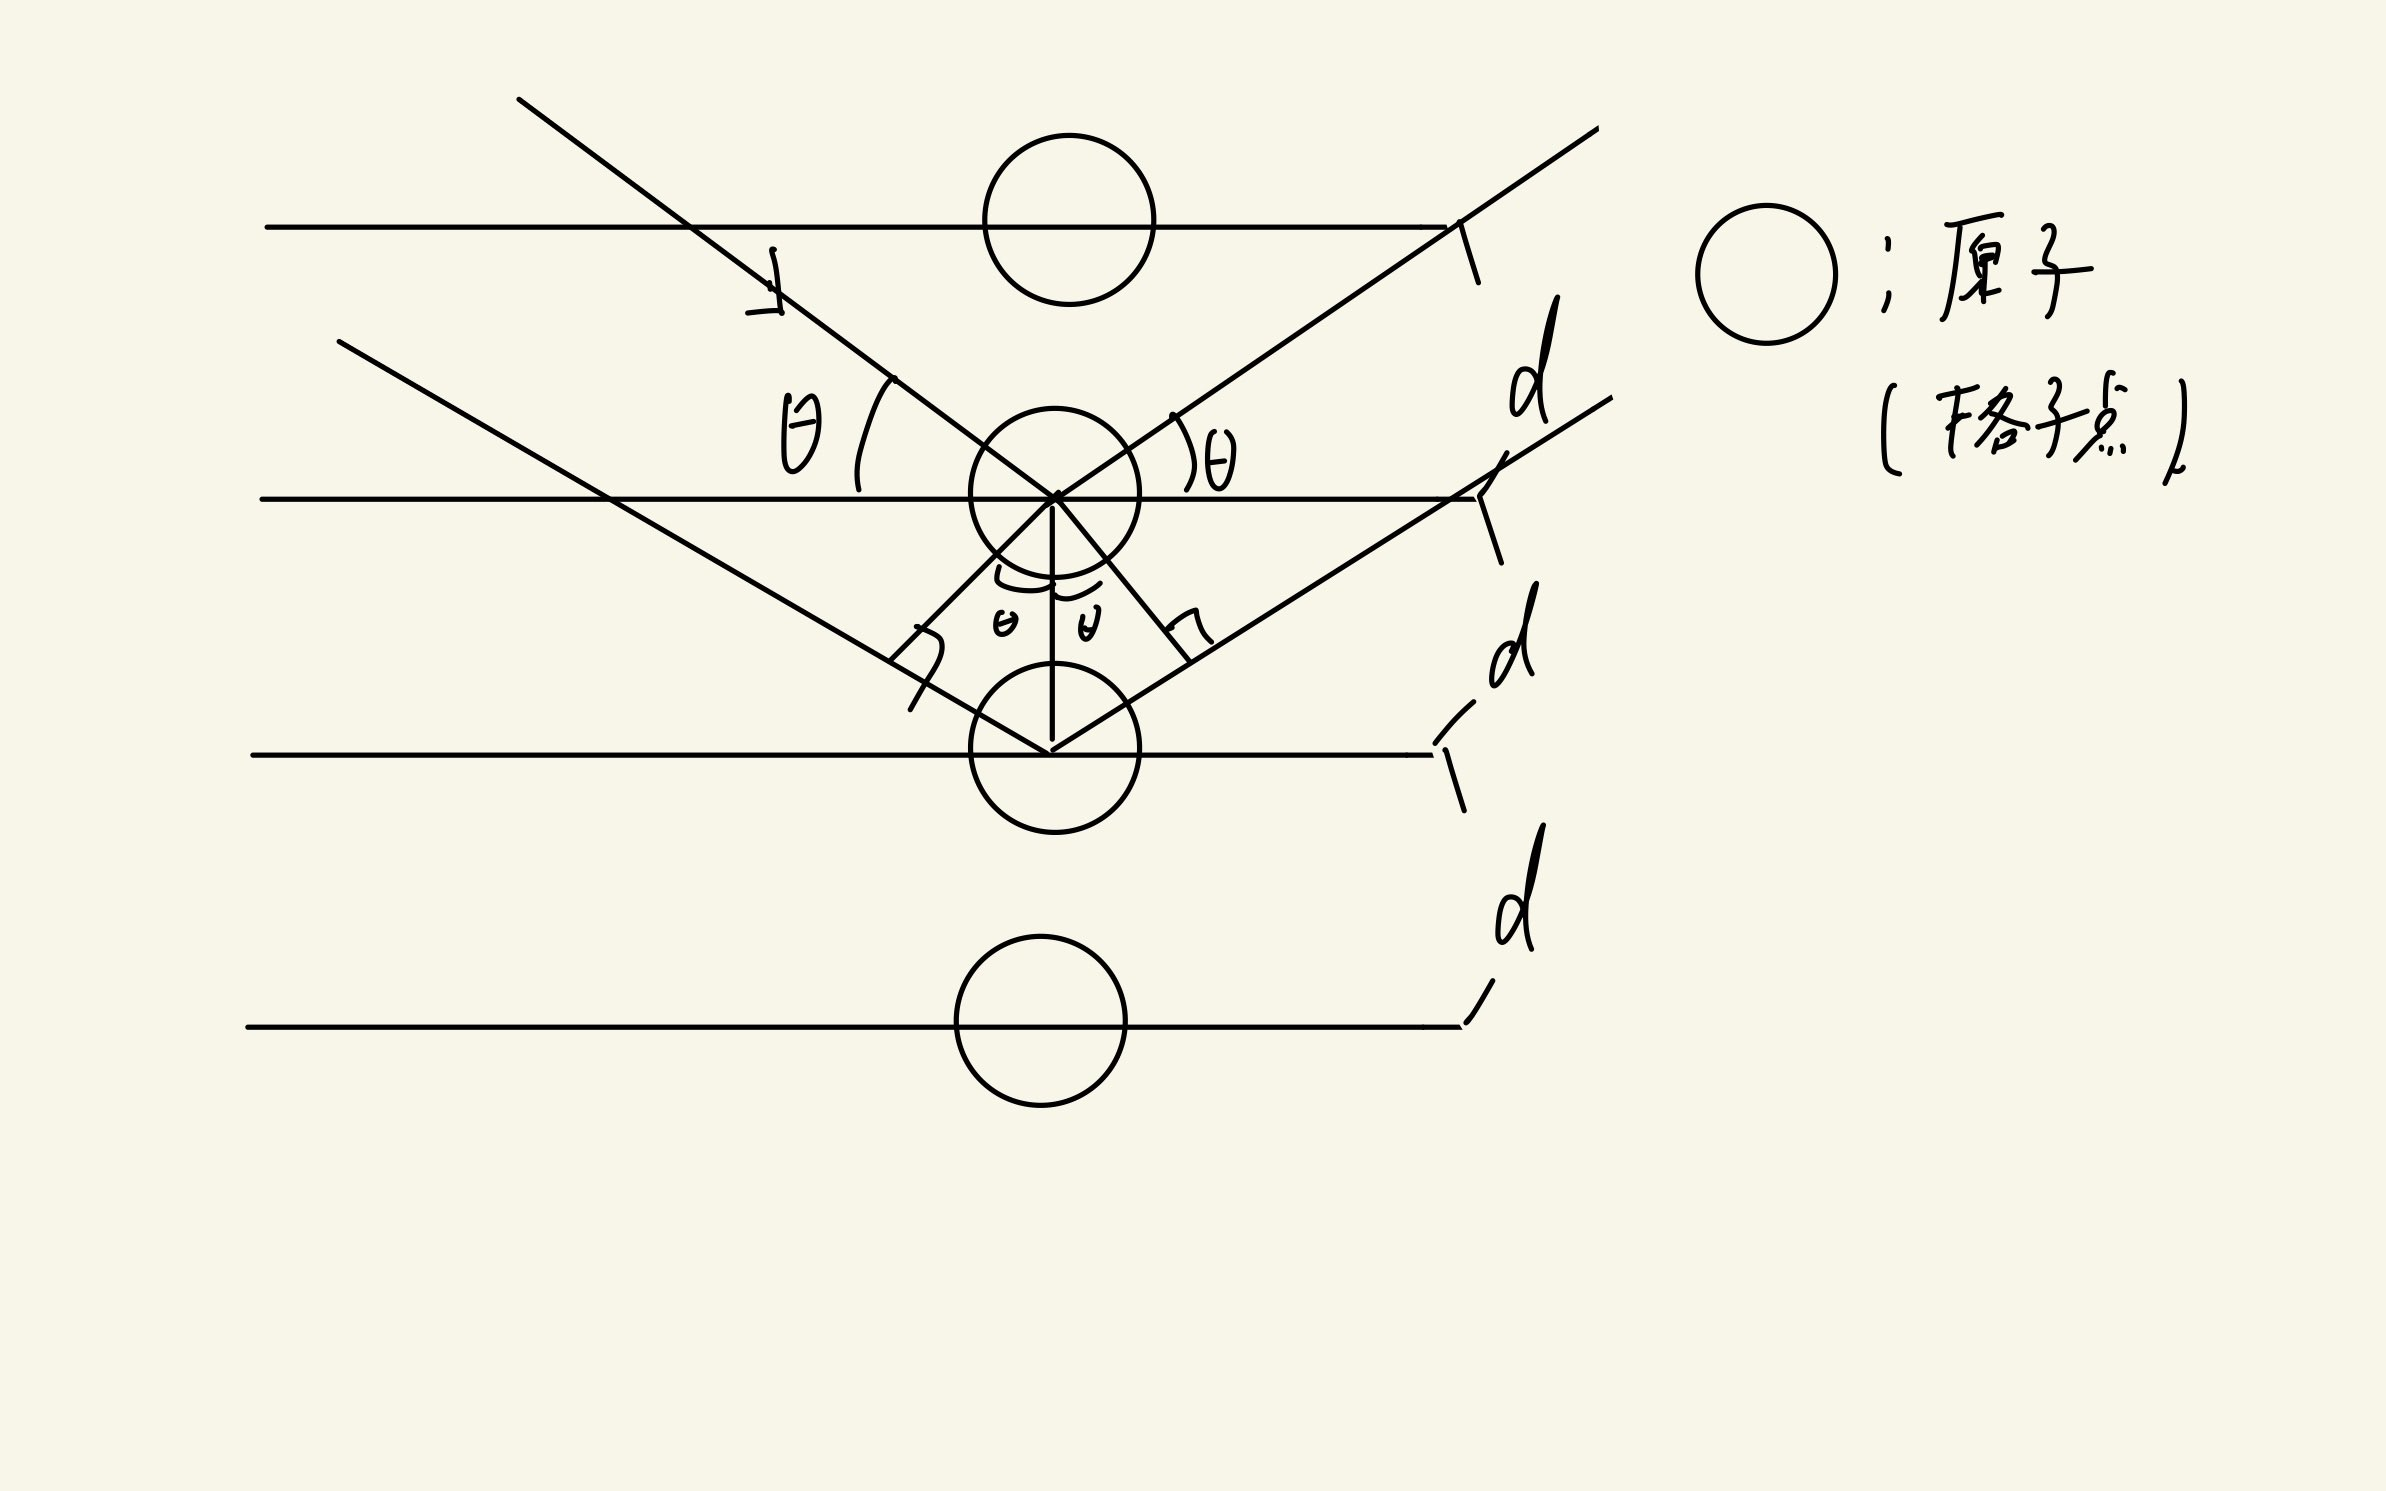
\includegraphics[width=100mm]{image2.jpg}
    \end{center}
    \caption{bragg}
    \label{fig:bragg}
\end{figure}

面間隔$d'$で隔てられた反射面に対し、$X$線が$\theta$の角度で入射するとき、隣り合う反射面で散乱された$X$線は$2d'\sin\theta$の光路差を持つ。
このとき、光路差が波長$\lambda$の整数倍のとき、散乱された$X$線は干渉を起こし、強度が増大する。すなわち、
\begin{align}
  2d'\sin\theta = n\lambda
\end{align}
が成り立つ。これをブラッグの条件という。
また、波長の$n$倍の光路差がある場合を、面間隔$d=\frac{d'}{n}$の場合として考えることができる。このとき、
\begin{align}
  2d\sin\theta = \lambda
\end{align}
が成り立つ。

\subsubsection{ブラべー格子}
3次元結晶格子において、結晶のパターンは14種類しかないことが知られている。これをブラベー格子という。これは、以下のようにまとめられる。
\begin{figure}[H]
    \begin{center}
    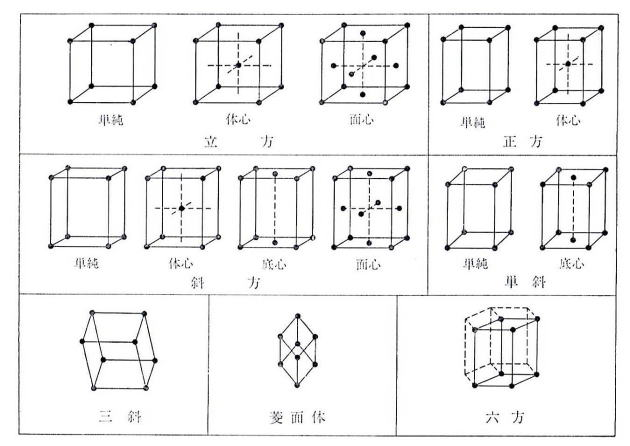
\includegraphics[width=80mm]{Bravais.jpg}
    \end{center}
    \caption{ブラベー格子}
    \label{fig:b}
\end{figure}

\subsubsection{ミラー指数と面間隔}
ミラー指数と呼ばれる指標を用いることで、反射面と面間隔の対応関係を考えることができる。
ミラー指数$(hkl)$で与えられる面は、$a/h$の位置で$a$軸と、$b/k$の位置で$b$軸と、$c/l$の位置で$c$軸と交わる面である。このとき、ミラー指数と面間隔の対応関係は以下の表のようになる。
\begin{table}[H]
  \centering
  \begin{tabular}{|c|c|}
    \hline
    結晶系 & 面間隔の式 \\ \hline
    単斜晶系 & $\frac{1}{d^2} = \frac{h^2}{a^2} + \frac{k^2}{b^2} + \frac{l^2}{c^2} - 2\frac{hl}{ac}\cos\beta$ \\ \hline
    斜方晶系 & $\frac{1}{d^2} = \frac{h^2}{a^2} + \frac{k^2}{b^2} + \frac{l^2}{c^2}$ \\ \hline
    正方晶系 & $\frac{1}{d^2} = \frac{h^2 + k^2}{a^2} + \frac{l^2}{c^2}$ \\ \hline
    立方晶系 & $\frac{1}{d^2} = \frac{h^2 + k^2 + l^2}{a^2}$ \\ \hline
    六方晶系 & $\frac{1}{d^2} = \frac{4}{3}\frac{h^2 + hk + k^2}{a^2} + \frac{l^2}{c^2}$ \\ \hline
  \end{tabular}
  \caption{結晶系と面間隔の関係}
  \label{tab:crystal_systems}
\end{table}

\subsubsection{構造因子}
格子点以外に置かれている原子によって散乱光が干渉を起こす場合が考えられる。この寄与を計算するために、構造因子と呼ばれる量を導入する。\\
図からわかるように
\begin{figure}[H]
    \begin{center}
    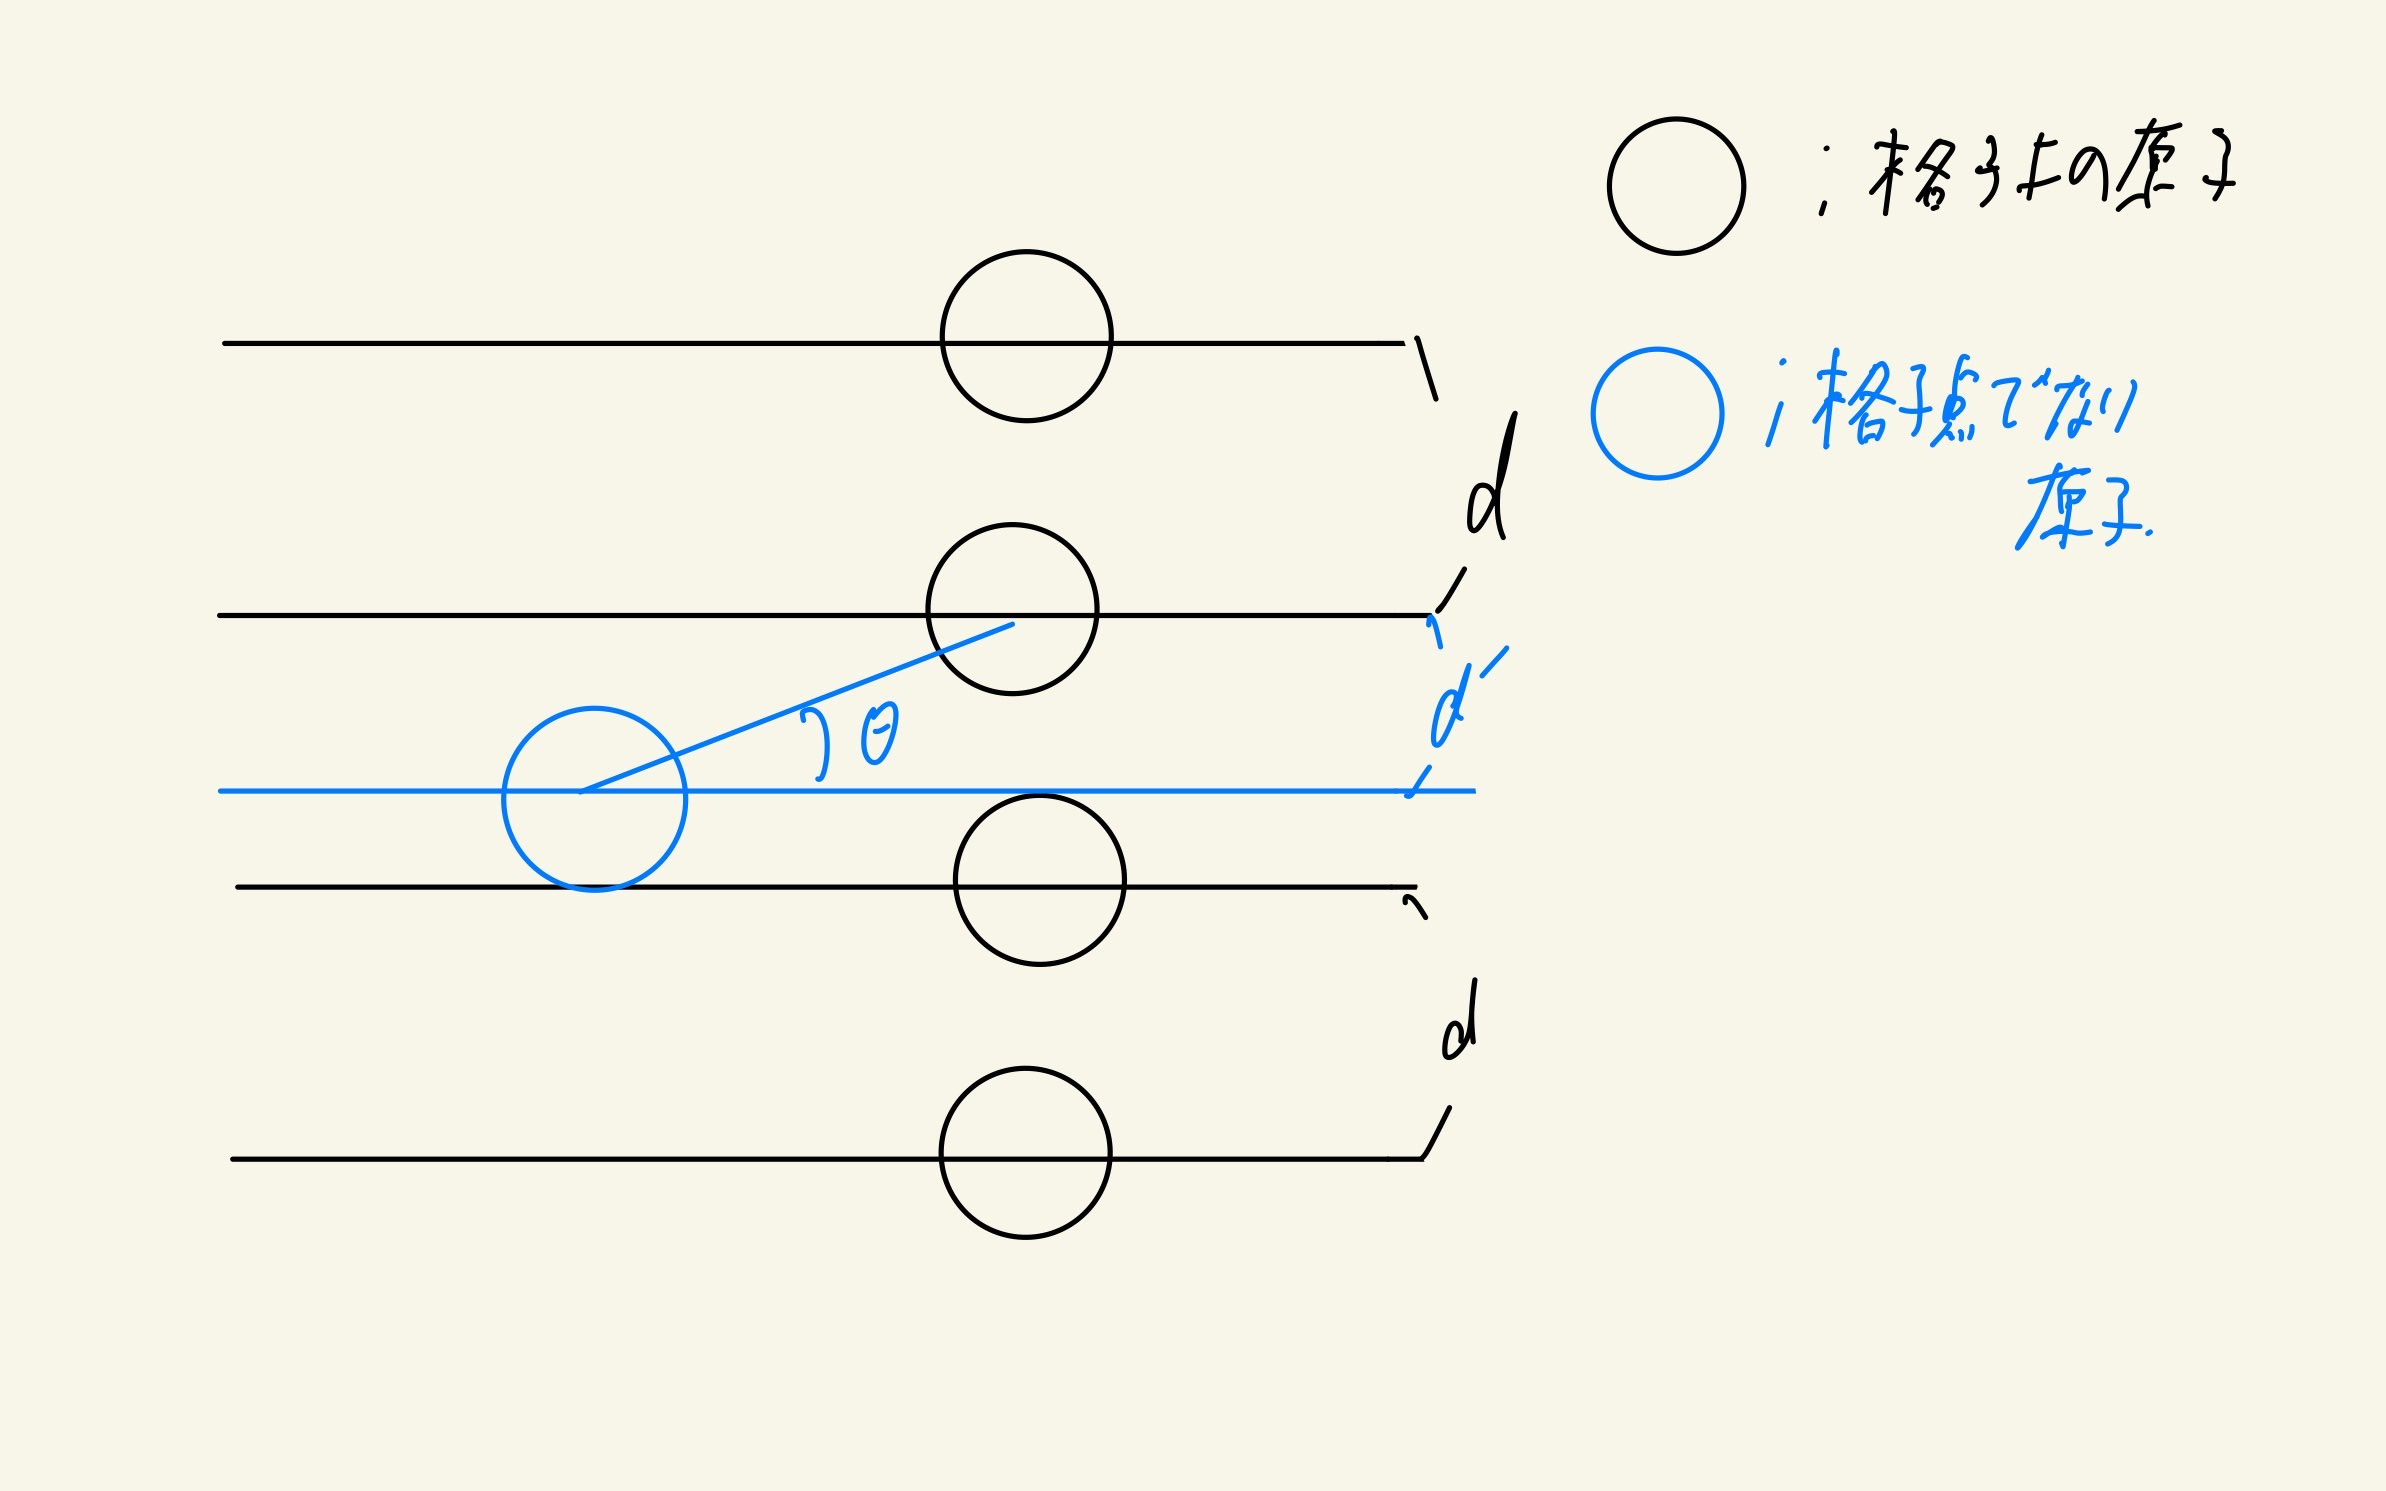
\includegraphics[width=100mm]{image.jpg}
    \end{center}
    \caption{構造因子}
    \label{fig:structure}
\end{figure}
隣り合う反射面の間の$d'$の位置にある原子からの散乱光と、格子点にある原子からの散乱光との光路差は$2d'\sin\theta$である。単位胞内にある原子の座標を$(u,v,w)$とすると、
$(h,k,l)$面に対しては、$2\pi(uh + vk + wl)$の位相差を持つ。これを、すべての単位胞内の原子について足し合わせることで、
\begin{align}
  F_{hkl} = \sum_{j}f_j\exp(2\pi i(u_jh + v_jk + w_jl))
\end{align}
が得られる。

\subsubsection{逆格子}
3つの独立な基底ベクトル$\bm{a}_1,\bm{a}_2,\bm{a}_3$を持つ格子に対して、それに双対な格子を考える。この格子を逆格子という。逆格子の基底ベクトルは、
\begin{align}
  \bm{b}_1 = 2\pi\frac{\bm{a}_2\times\bm{a}_3}{\bm{a}_1\cdot(\bm{a}_2\times\bm{a}_3)} \\
  \bm{b}_2 = 2\pi\frac{\bm{a}_3\times\bm{a}_1}{\bm{a}_1\cdot(\bm{a}_2\times\bm{a}_3)} \\
  \bm{b}_3 = 2\pi\frac{\bm{a}_1\times\bm{a}_2}{\bm{a}_1\cdot(\bm{a}_2\times\bm{a}_3)}
\end{align}
で与えられる。また、一般の逆格子は、
\begin{align}
  \bm{H} = h\bm{b}_1 + k\bm{b}_2 + l\bm{b}_3
\end{align}
で表される。\\
このことを用いてブラッグの反射条件を表すことを考える。このとき、入射方向の単位ベクトルを$\bm{s}_0$、散乱方向の単位ベクトルを$\bm{s}$とすると、
\begin{align}
  \bm{H} = \frac{\vb{s}_0 - \vb{s}}{\lambda} \label{eq:bragg}
\end{align}
が成り立つ。この式は、ラウエの式と呼ばれる。\\
また、構造因子についても内積を使った簡潔に書き直すことができ、
\begin{align}
  F_{hkl} = \sum_{j}f_j\exp(2\pi i\bm{H}\cdot\bm{r}_j)
\end{align}
と書くことができる。すなわち、電子分布の離散Fourier逆変換となる。

\subsubsection{エバルト球}
$X$線を散乱する資料を中心Pにとった、半径$\frac{1}{\lambda}$の球のことをエバルト反射球と呼ぶ。この球を用いると、散乱ベクトルと逆格子点の関係を考えることができる。
エバルト球は、結晶の回折条件を視覚的に理解するための便利なツールである。エバルト球の半径は$1/\lambda$であり、球の中心は入射波ベクトル$\bm{k}_0$の先端に位置する。エバルト球の表面上に逆格子点が存在する場合、その点に対応する反射が観測される。

エバルト球の構成は以下の通りである:
\begin{enumerate}
  \item 入射波ベクトル$\bm{s}_0$の長さは$1/\lambda$であり、結晶の原点から始まる。
  \item 散乱波ベクトル$\bm{s}$も長さ$1/\lambda$であり、エバルト球の表面上に終わる。
  \item 逆格子ベクトル$\bm{H}$は、エバルト球の中心から逆格子点までのベクトルである。
\end{enumerate}

エバルト球の条件を満たすためには、以下のベクトル関係が成り立つ必要がある。
\begin{align}
  \bm{s} = \bm{s}_0 + \bm{H}
\end{align}

この条件を満たす逆格子点がエバルト球の表面上に存在する場合、その点に対応する反射が観測される。エバルト球を用いることで、結晶の回折条件を視覚的に理解しやすくなる。
%推敲済み

\subsection{ラウエ法}
上で説明した反射球を回転させることで、逆格子点に対応する反射を観測することができる。
試料で散乱された$X$線の方向が(\ref{eq:bragg})のように逆格子ベクトルと関係していることから、ラウエ写真には逆格子に対応する斑点(ラウエ斑点)が現れる。これの位置関係から逆格子ベクトルの方向を決定することができる。
このような実験手法のことをラウエ法という。

\subsubsection{グレニンガーチャート・レオンハルトチャート}
逆フーリエ変換などを用いても逆格子ベクトルの方向を決めることはできるのであるが、基本的に計算が煩雑になってしまう。それを避けるための手法として、
以下の図のようなグレニンガーチャートやレオンハルトチャートを用いることがある。
\begin{figure}[H]
    \begin{center}
    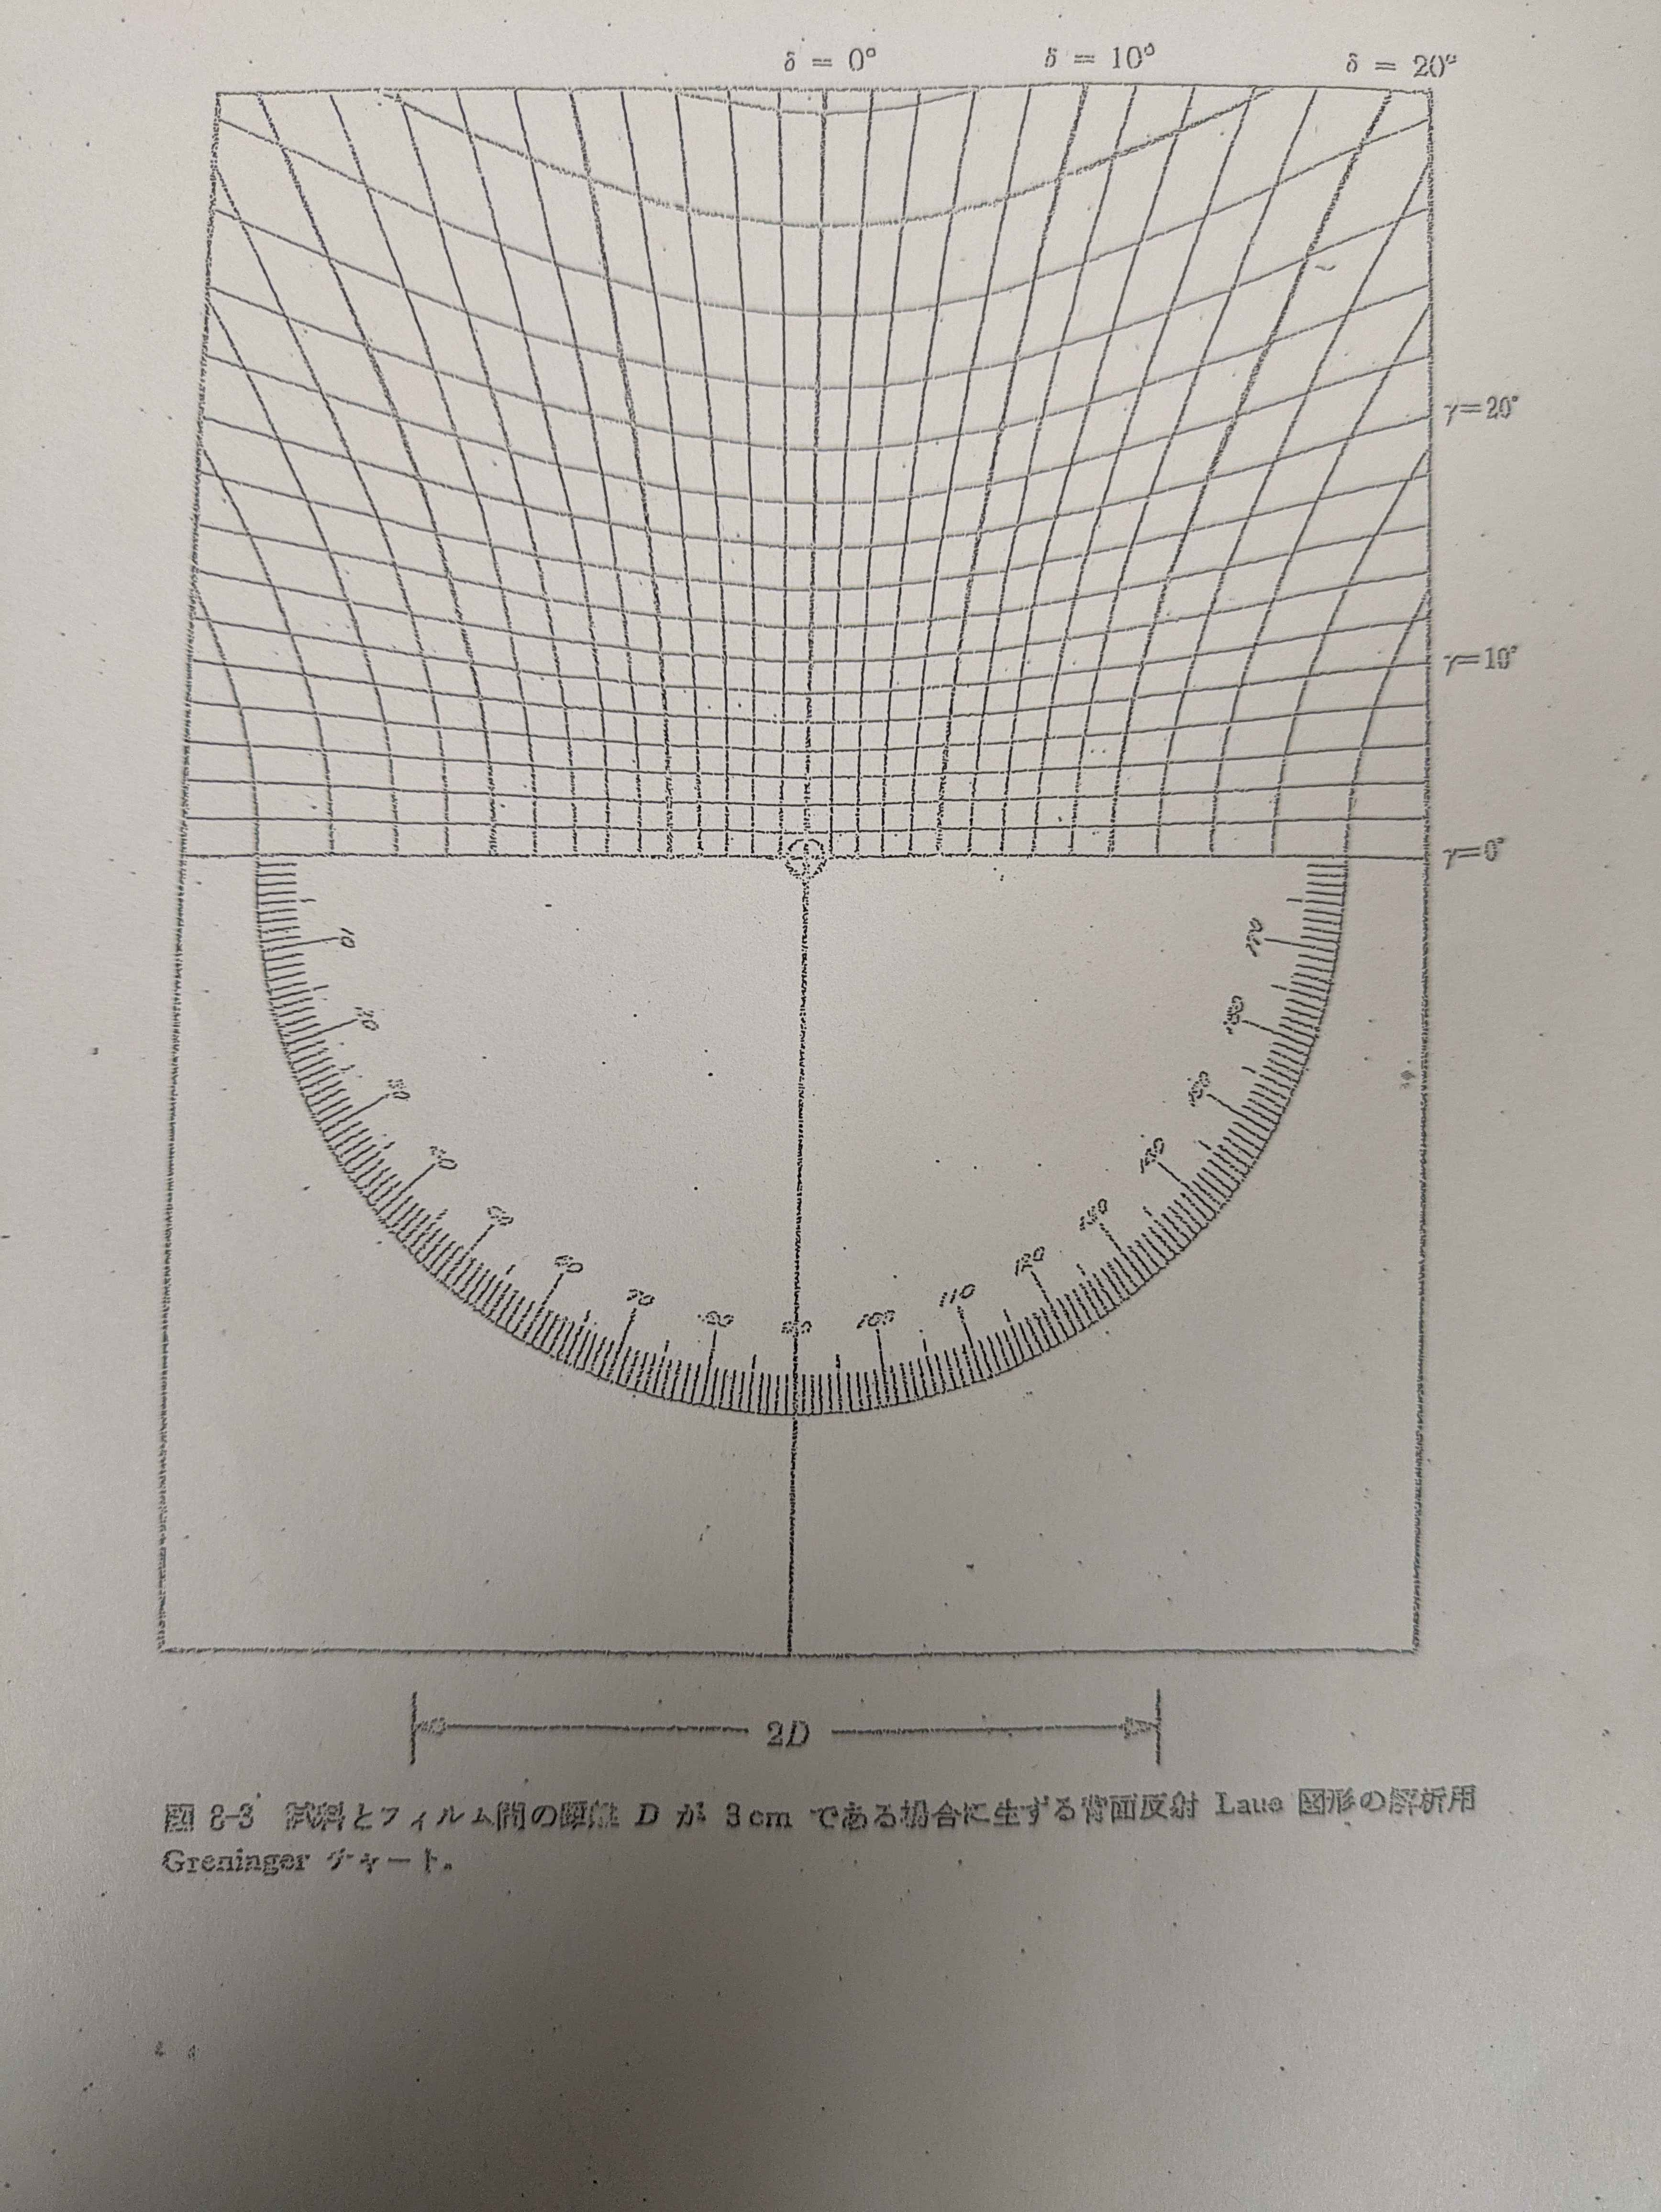
\includegraphics[width=80mm]{g.jpg}
    \end{center}
    \caption{グレニンガーチャート}
    \label{fig:g}
\end{figure} 
これらのチャートには、極座標で表される逆格子ベクトルの方向$(\delta,\gamma)$がプロットされている。

\subsubsection{ステレオ投影とウルフネット}
3次元的なベクトルを2次元に埋め込むために、ウルフネットを用いる。これは、等$\delta$線と等$\gamma$線を描くことで、逆格子ベクトルの方向を表現するものである。
\begin{figure}[H]
    \begin{center}
    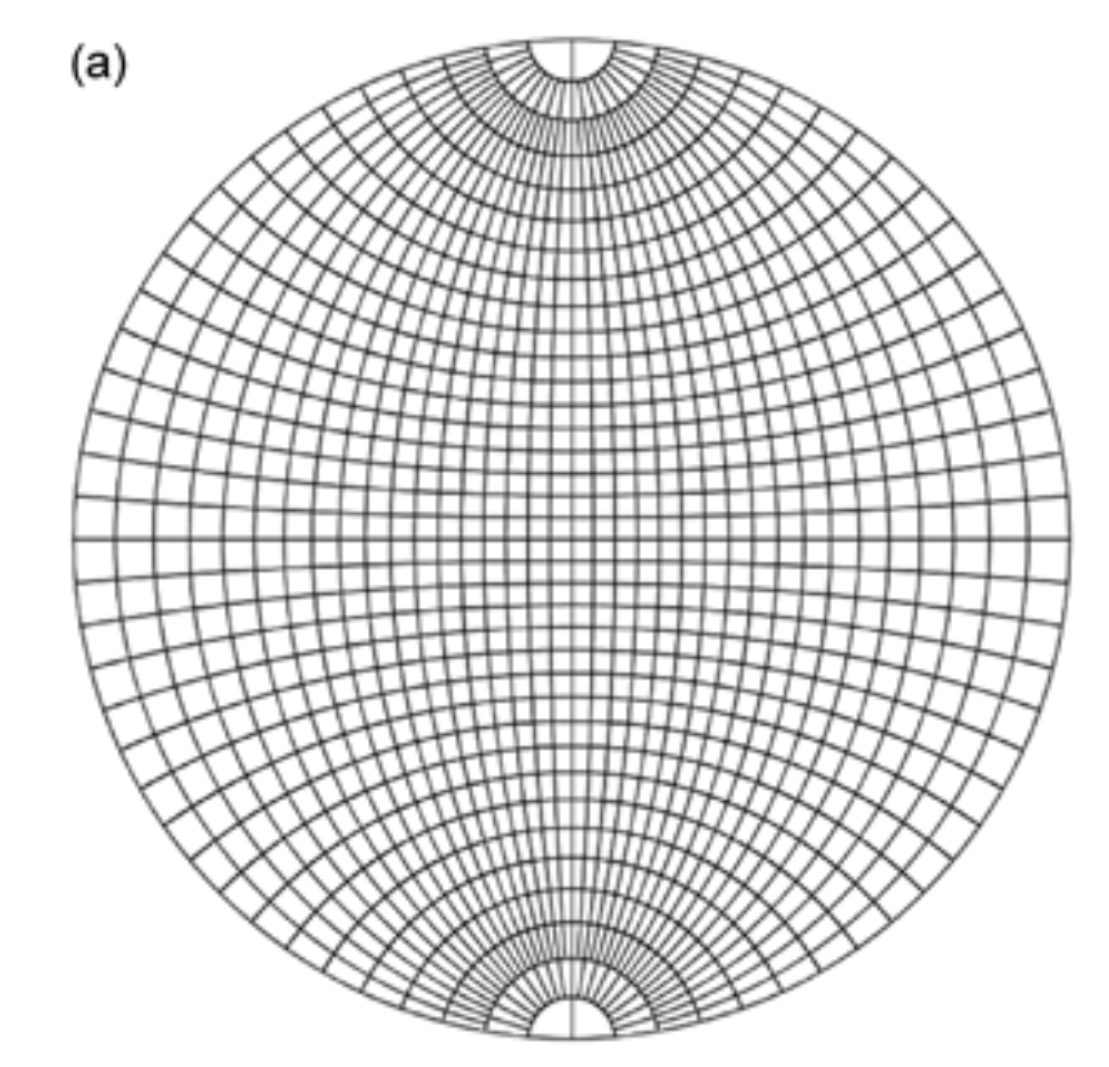
\includegraphics[width=100mm]{u.png}
    \end{center}
    \caption{ウルフネット}
    \label{fig:u}
\end{figure}

\subsubsection{標準投影図}
重要な結晶面を投影面としたときの投影図のことを標準投影図という。本実験では、実験データとこの投影図を比較して、実験結果を精査する。
\begin{figure}[H]
    \begin{center}
    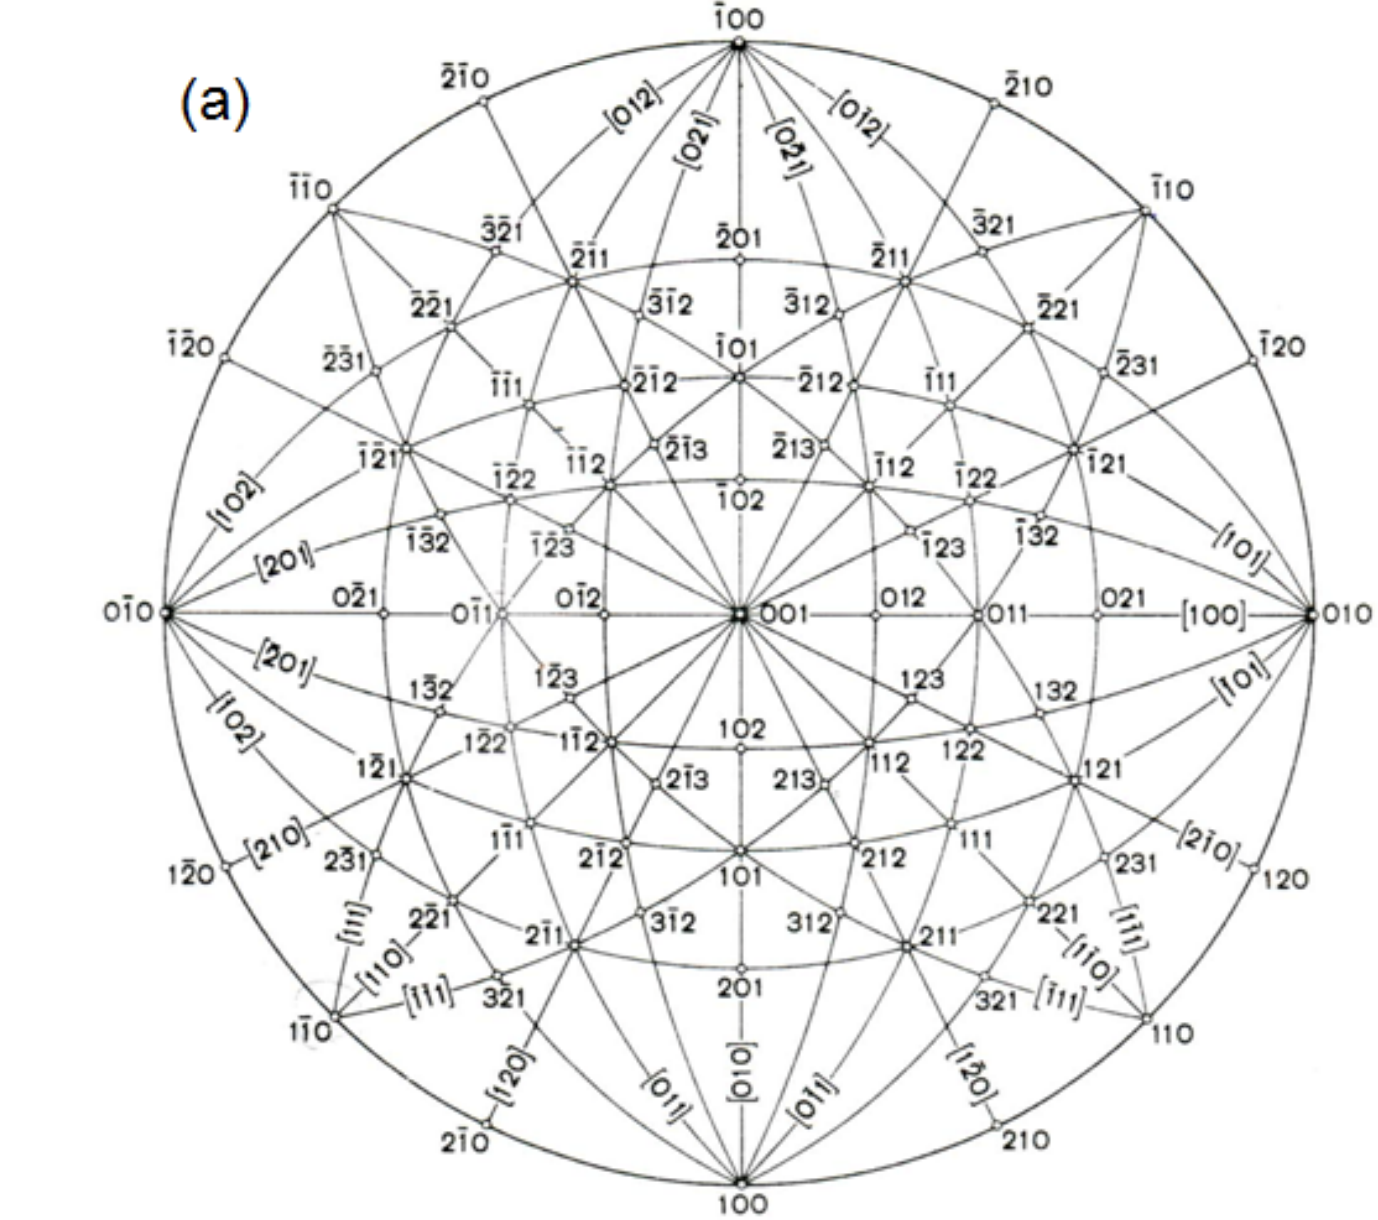
\includegraphics[width=80mm]{standard.png}
    \end{center}
    \caption{標準投影図}
    \label{fig:standard}
\end{figure}
%推敲済み

\section{方法}
\begin{enumerate}
  \item X線の出力を30kV, 15mAに設定し、約15分間露光することでラウエ写真を撮影した。ただし、試料からイメージングプレートまでの距離を30mmとした。
  \item 実験結果を印刷し、グレニンガーチャートやウルフネットを用いて解析を行った。
\end{enumerate}
%推敲済み

\section{結果}
\subsection{001型結晶}
以下の001型結晶のラウエ写真を撮影した。
\begin{figure}[H]
  \centering
  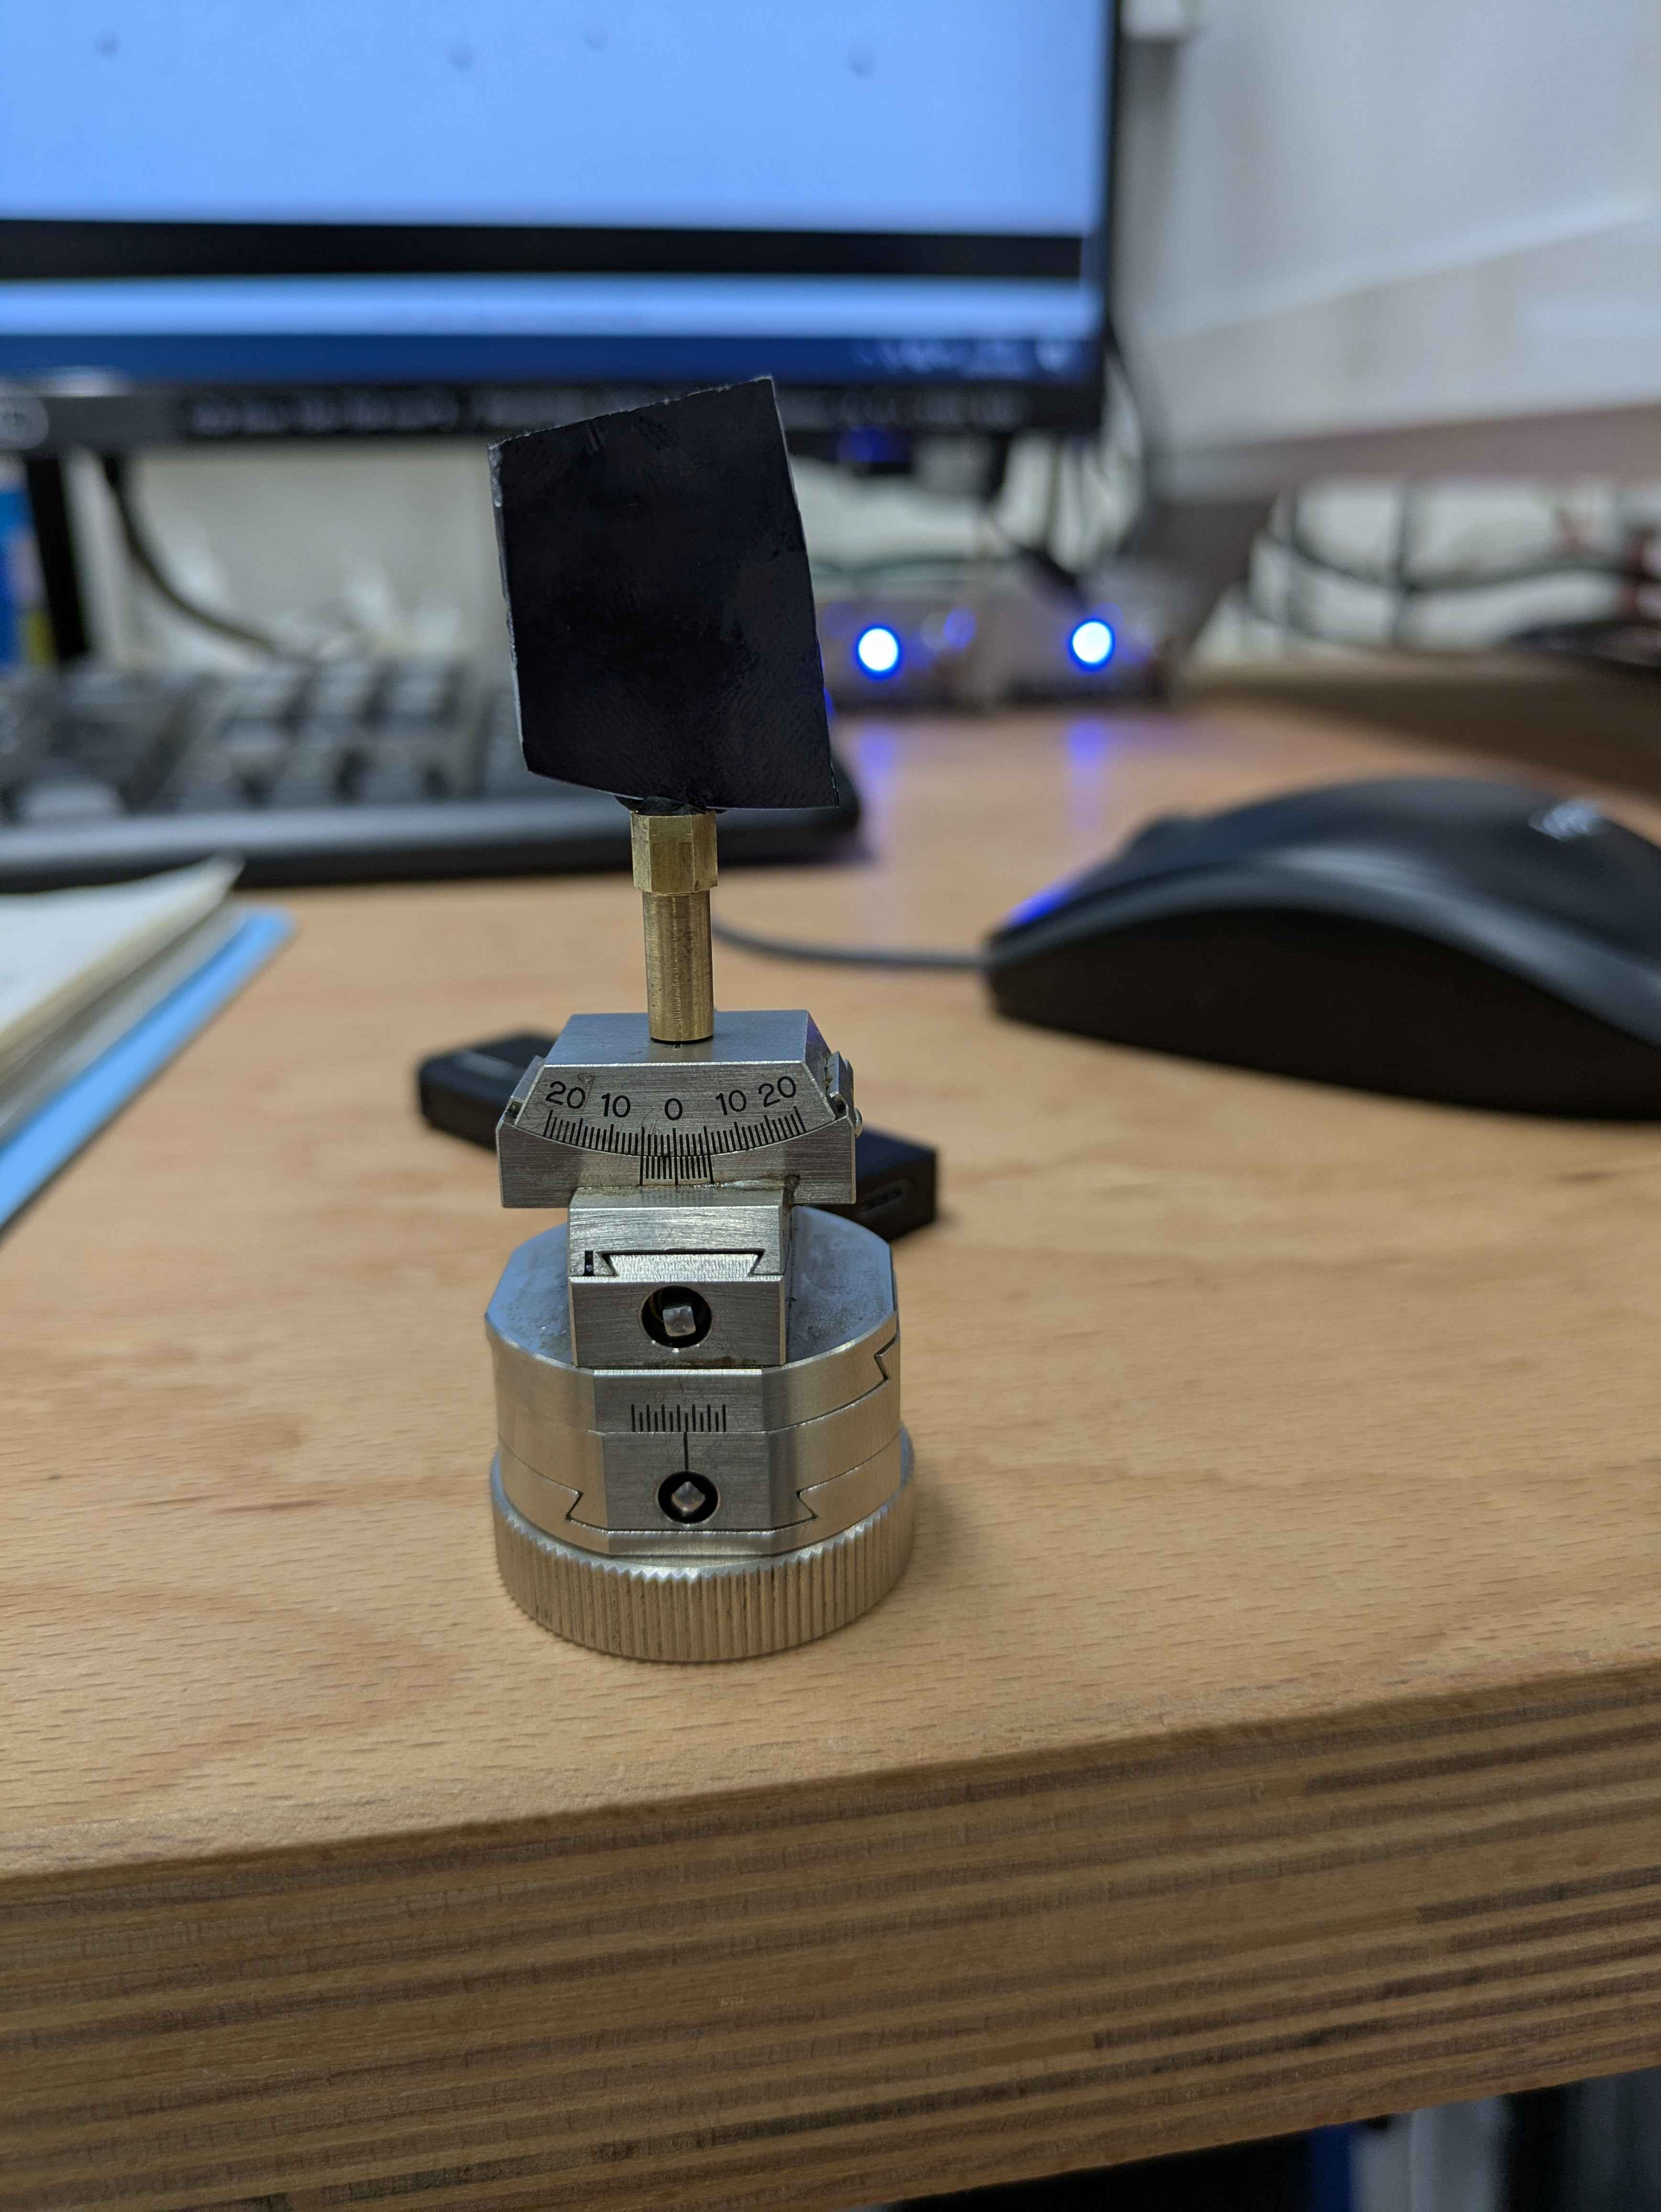
\includegraphics[width=6cm]{mae.jpg}
  \caption{001型結晶のラウエ写真}
\end{figure}

このとき、ラウエ写真は以下のようになった。
\begin{figure}[H]
  \centering
  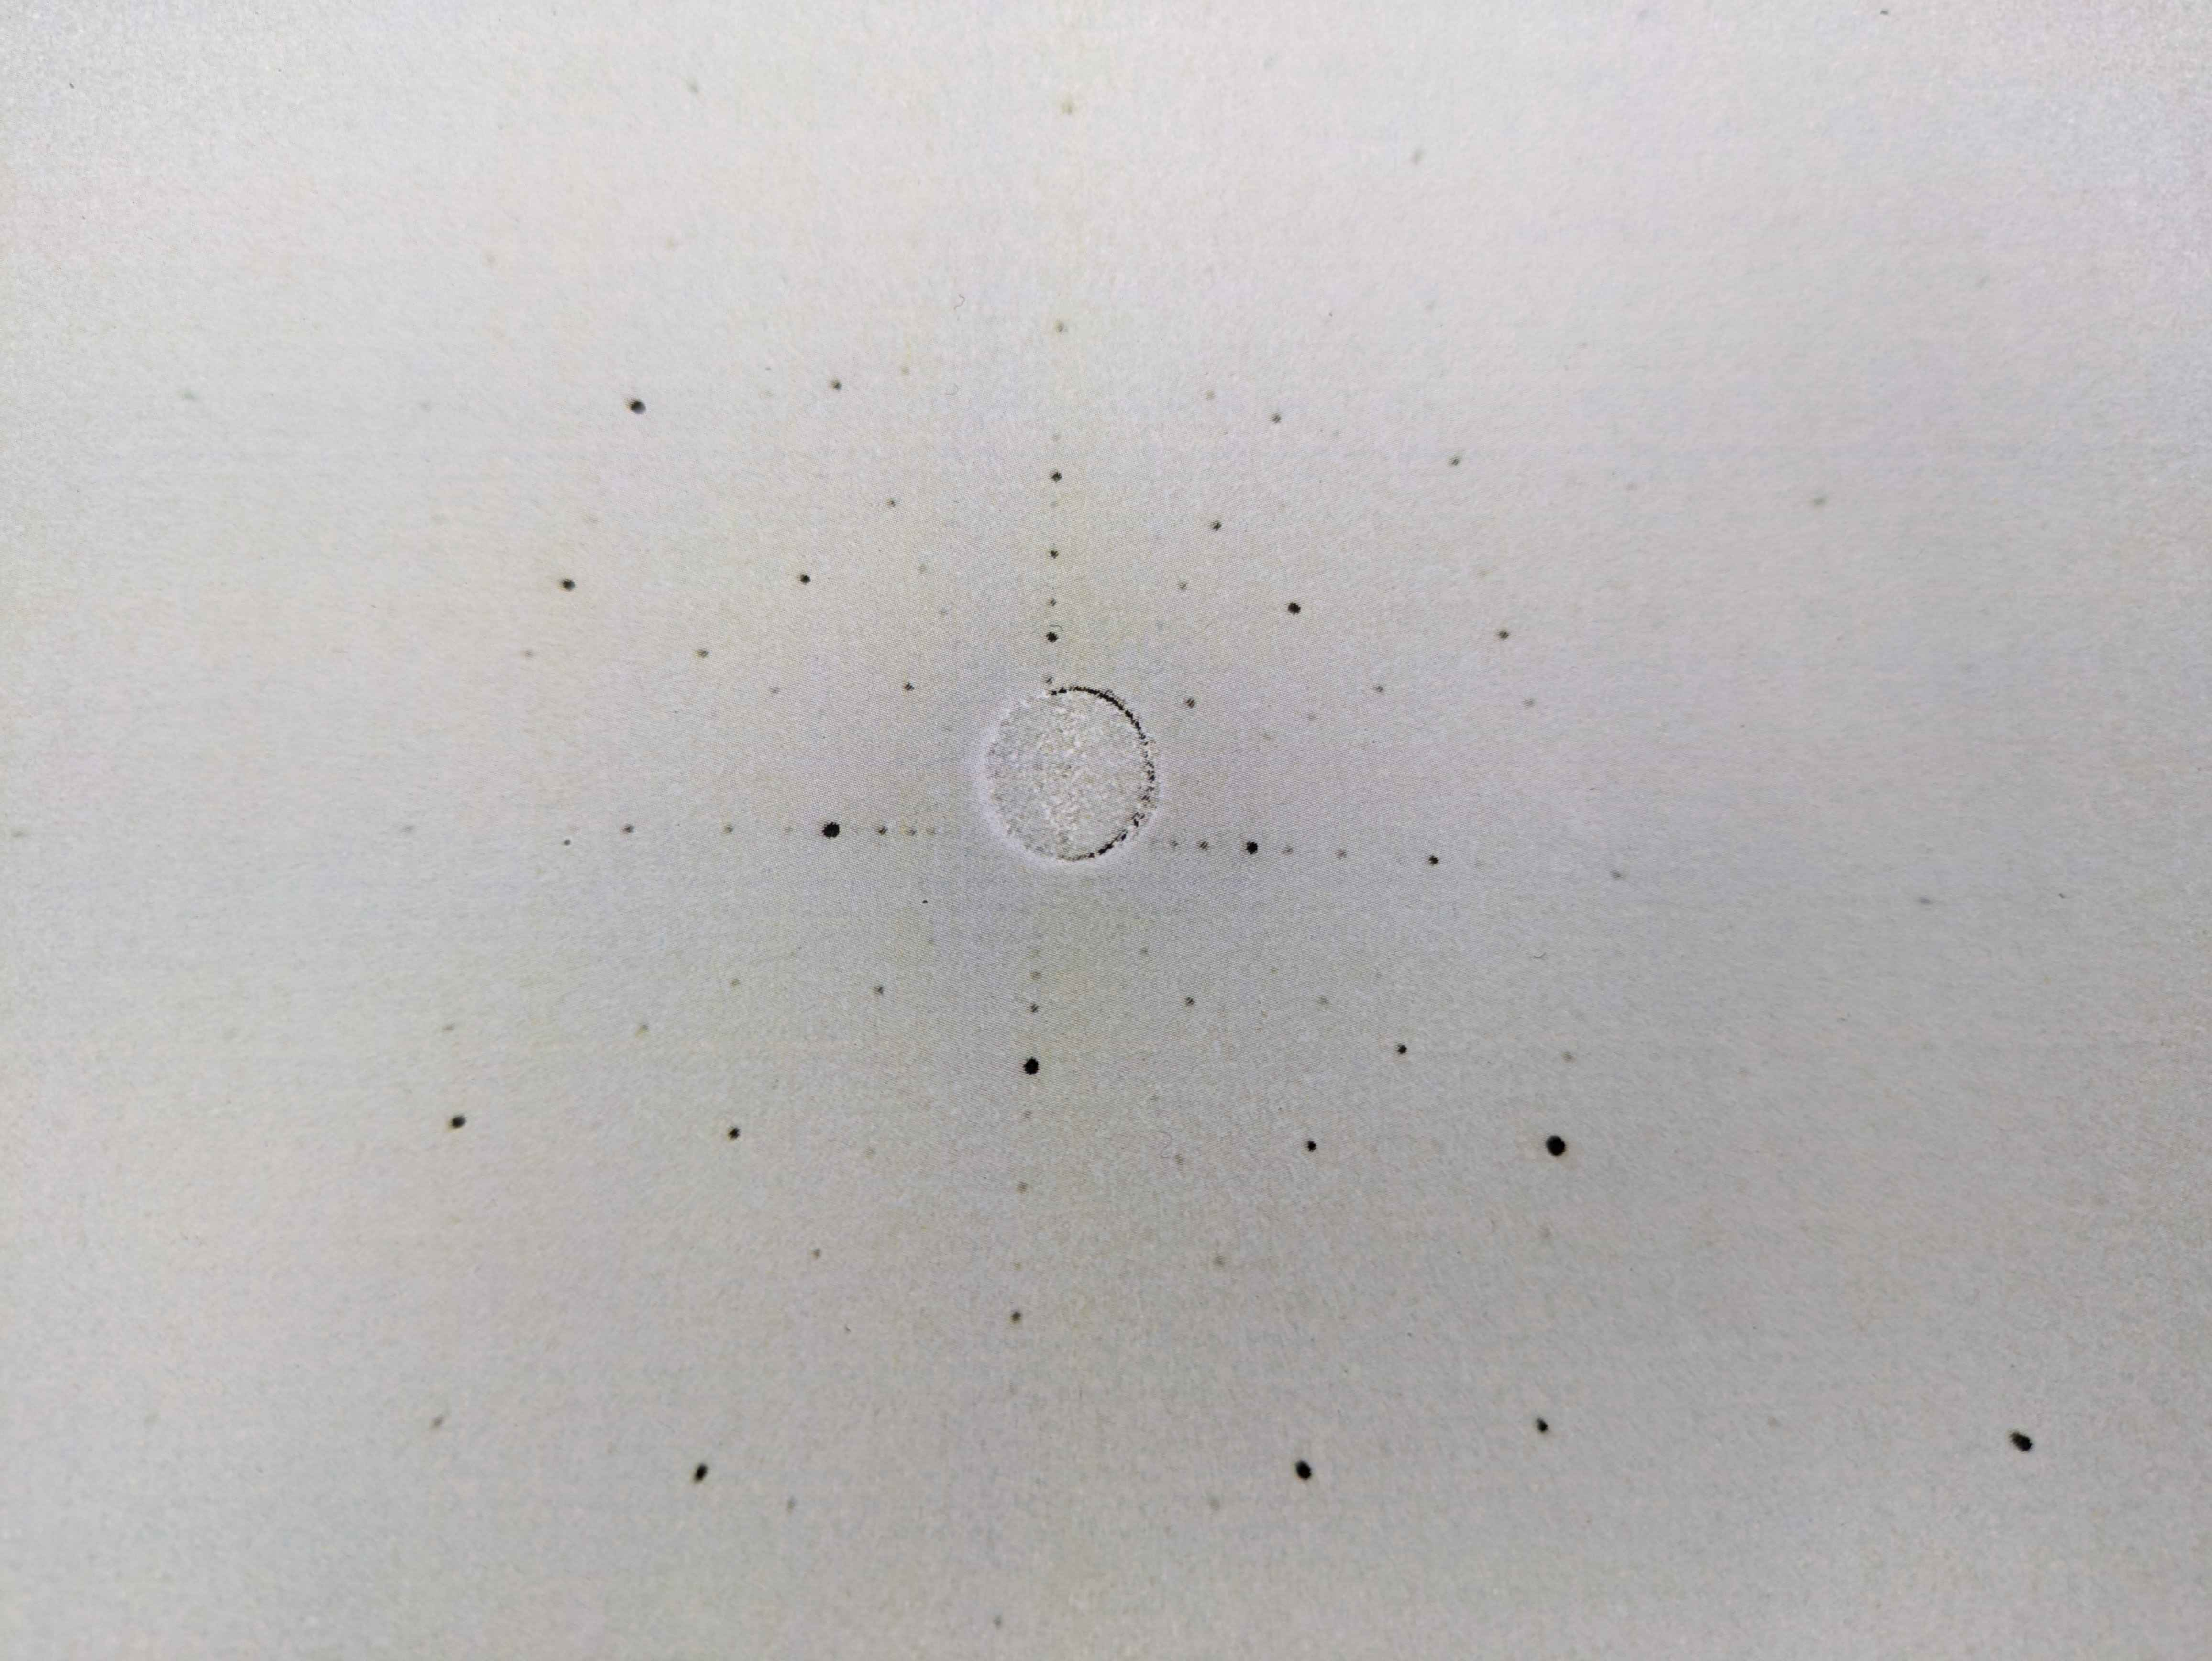
\includegraphics[width=6cm]{001.jpg}
  \caption{001型結晶のラウエ写真}
\end{figure}


\subsection{111型結晶}
以下の111型結晶のラウエ写真を撮影した。
\begin{figure}[H]
  \centering
  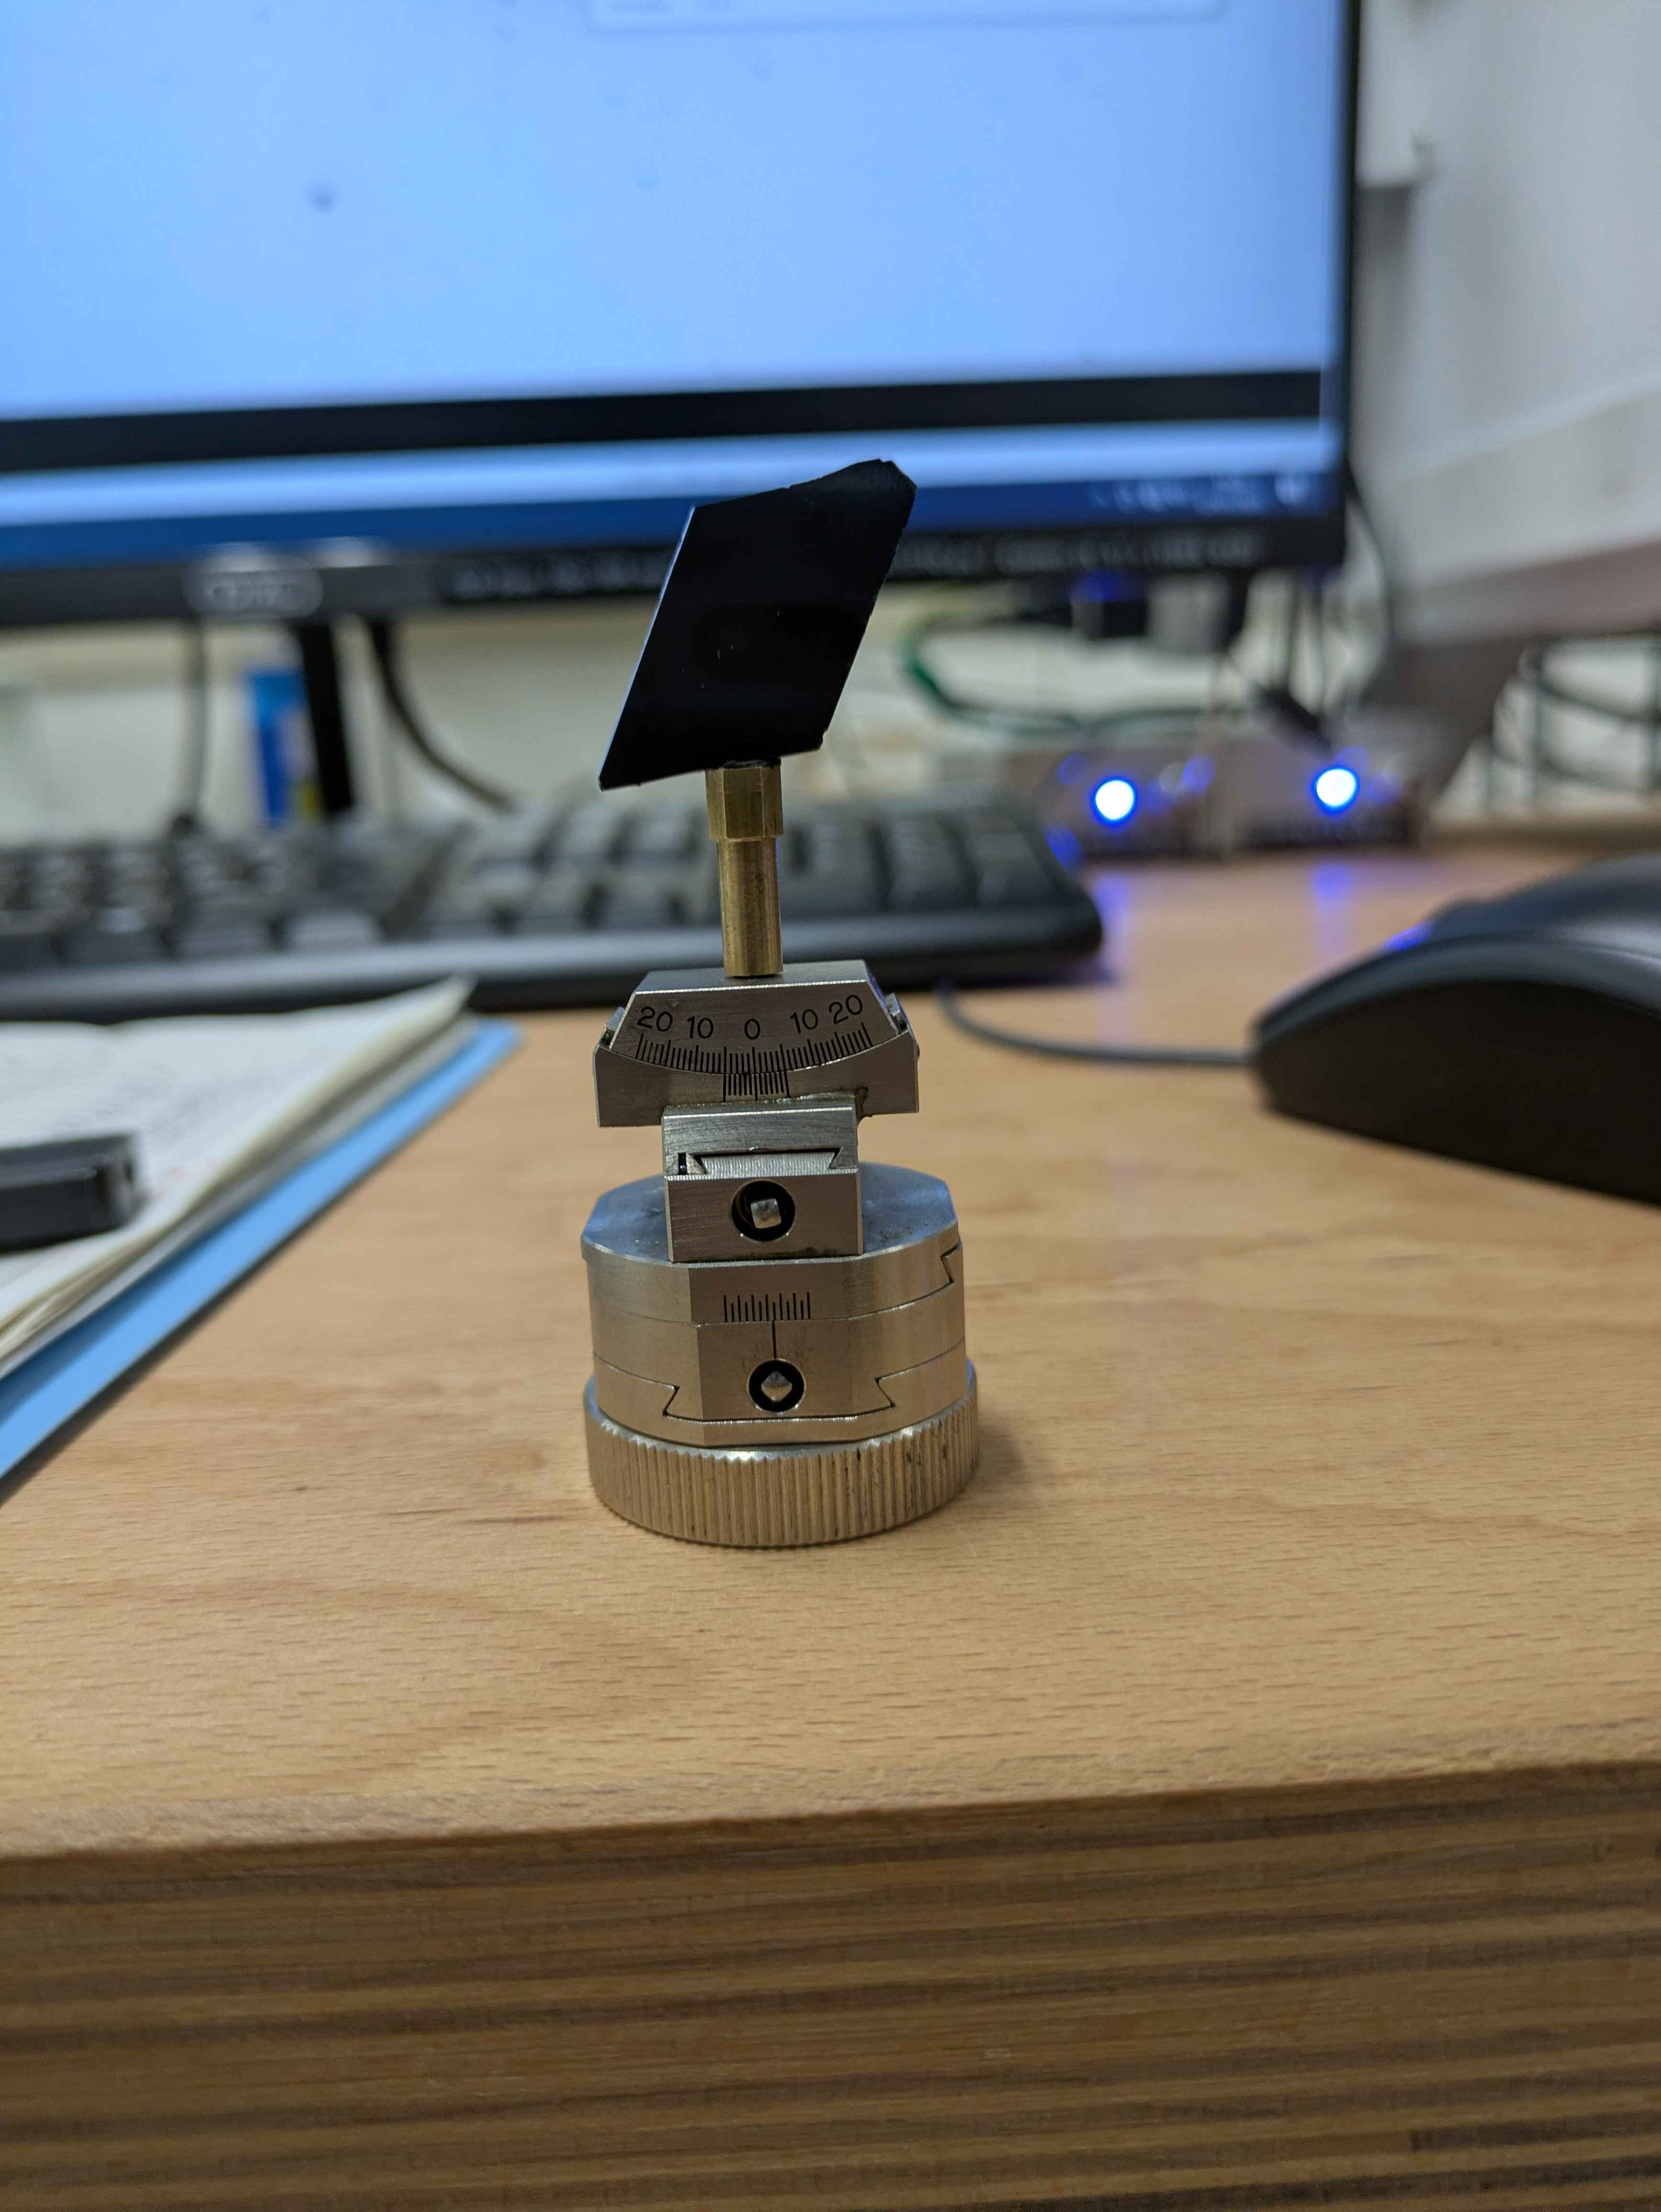
\includegraphics[width=6cm]{ato.jpg}
  \caption{111型結晶のラウエ写真}
\end{figure}

このとき、ラウエ写真は以下のようになった。
\begin{figure}[H]
  \centering
  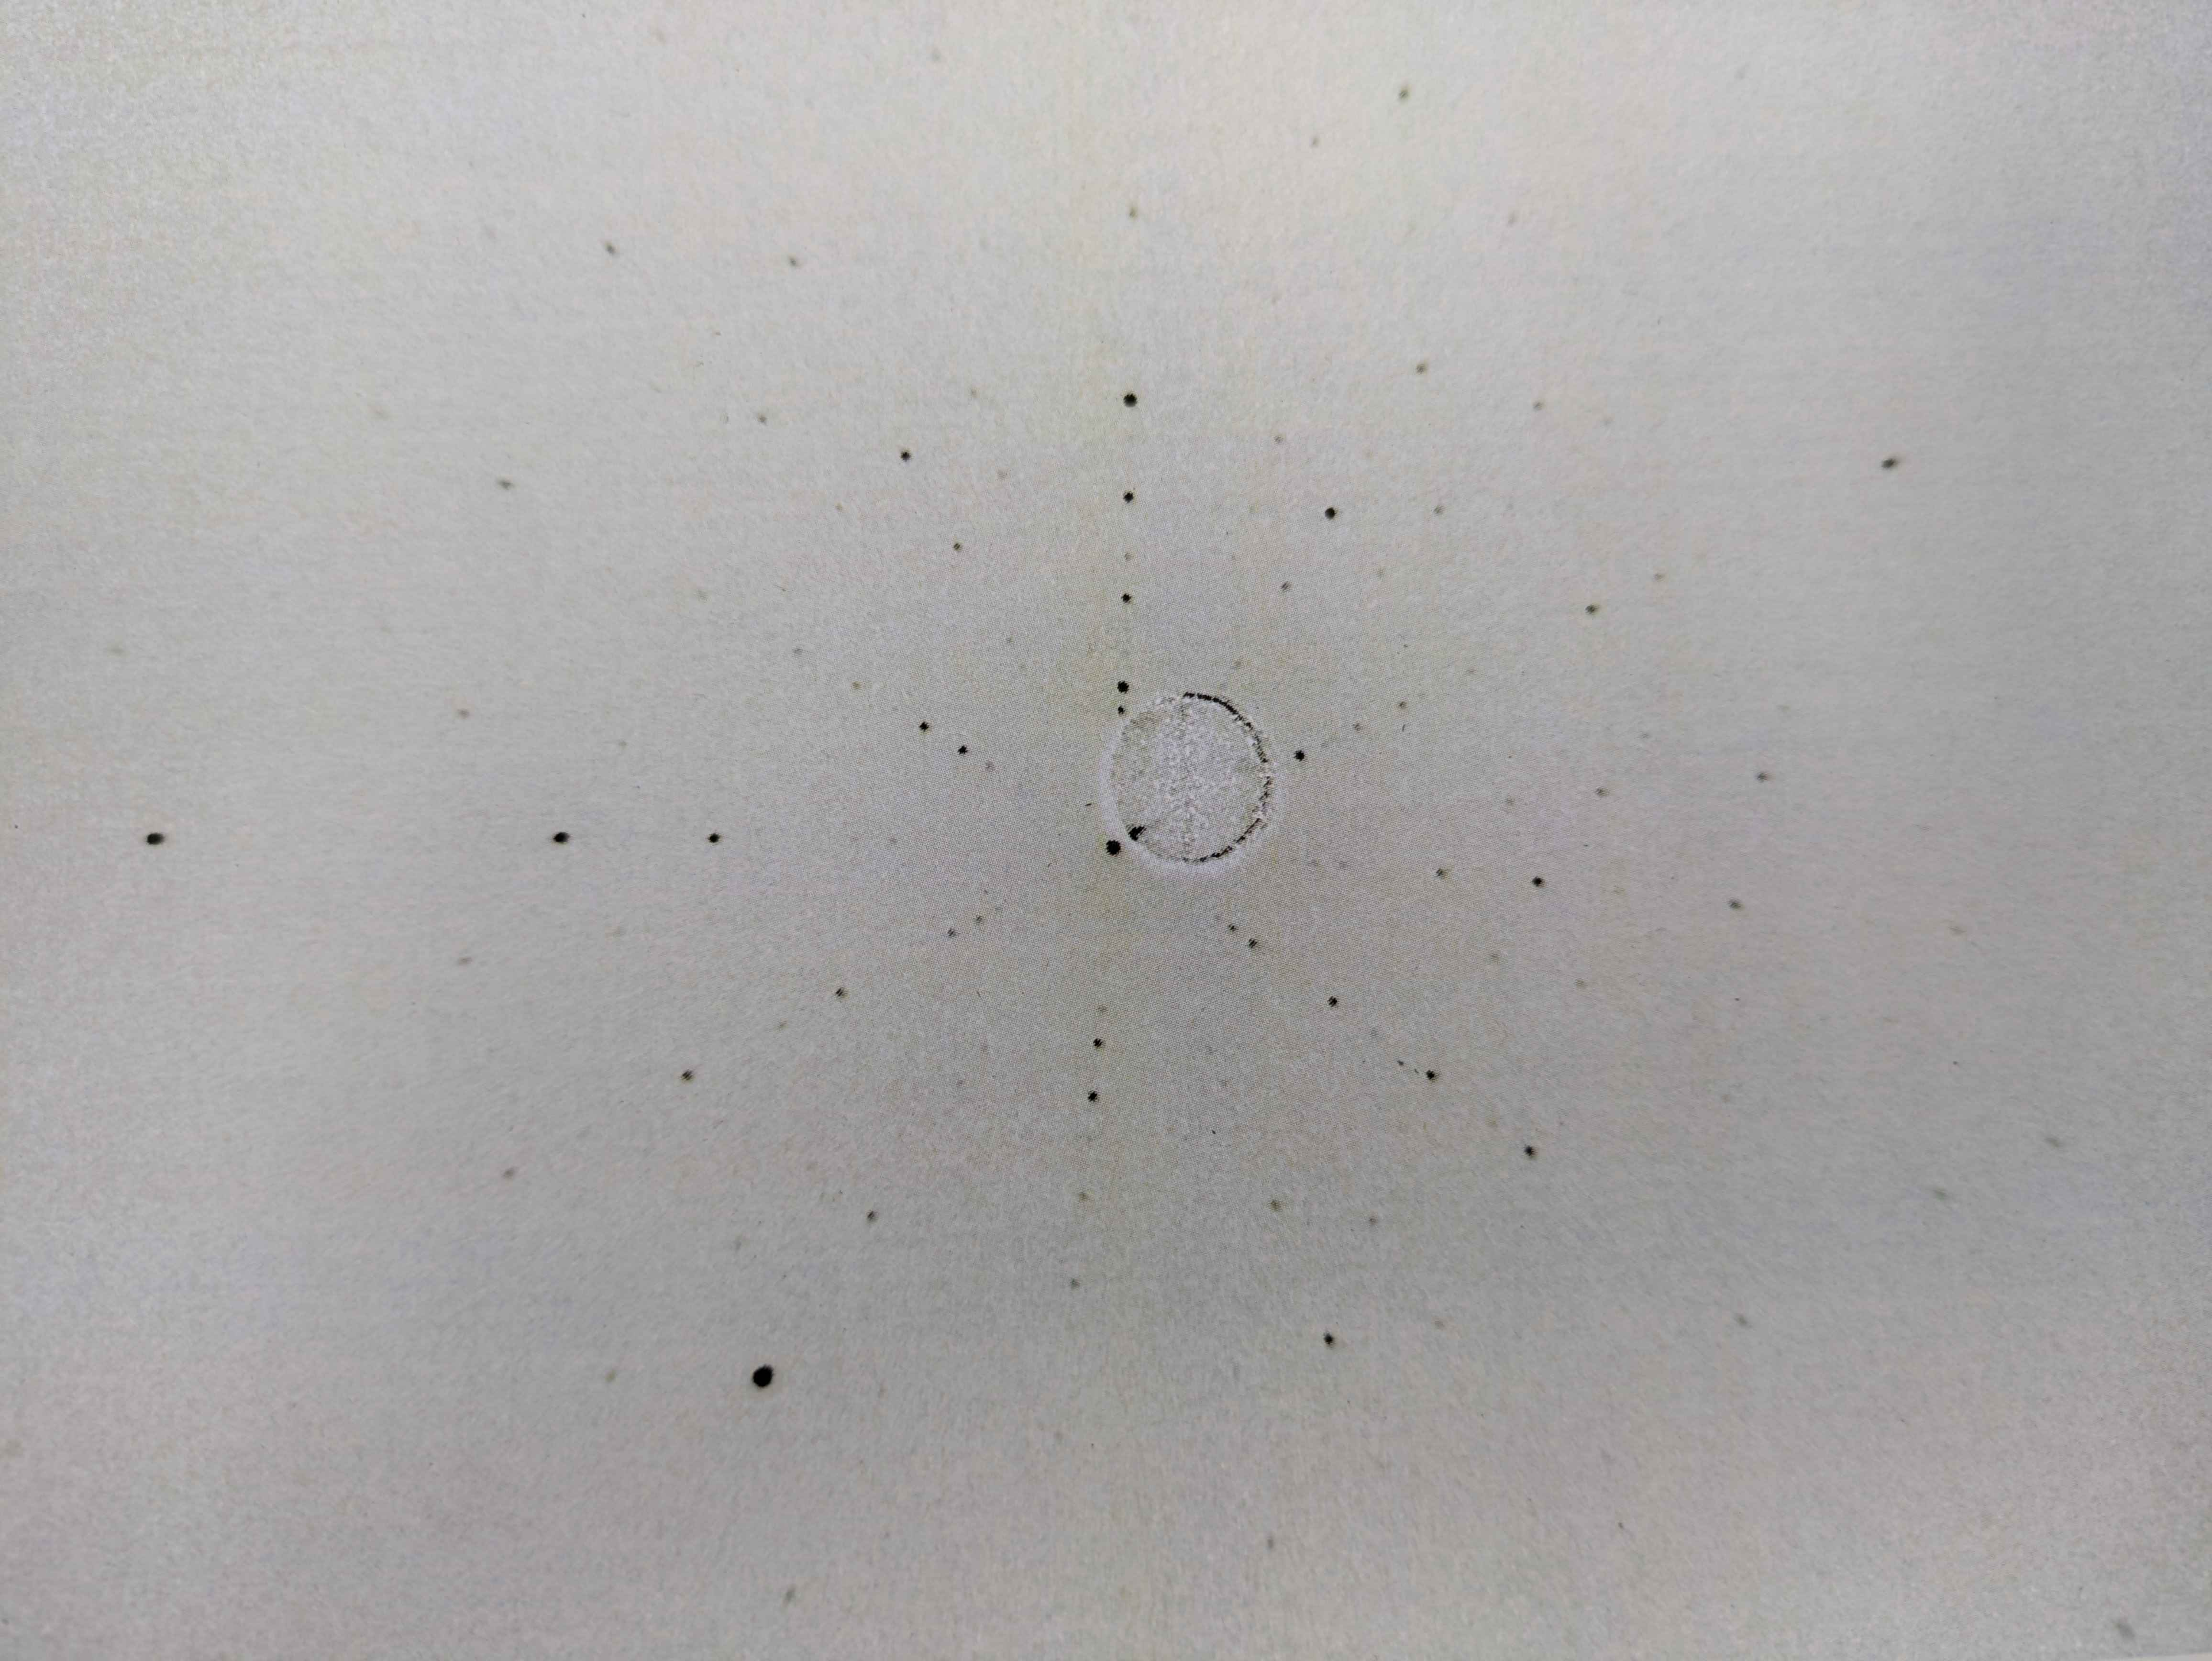
\includegraphics[width=6cm]{110.jpg}
  \caption{111型結晶のラウエ写真}
\end{figure}
%推敲済み


\section{考察}
\subsection{001型結晶}
001型結晶について、Wulfネットを用いて解析を行った。

\subsubsection{グレニンガーチャート}
グレニンガーチャートをトレースシートに重ねて、逆格子ベクトルの方向を決定した。この結果は以下のようになった。
\begin{figure}[H]
  \centering
  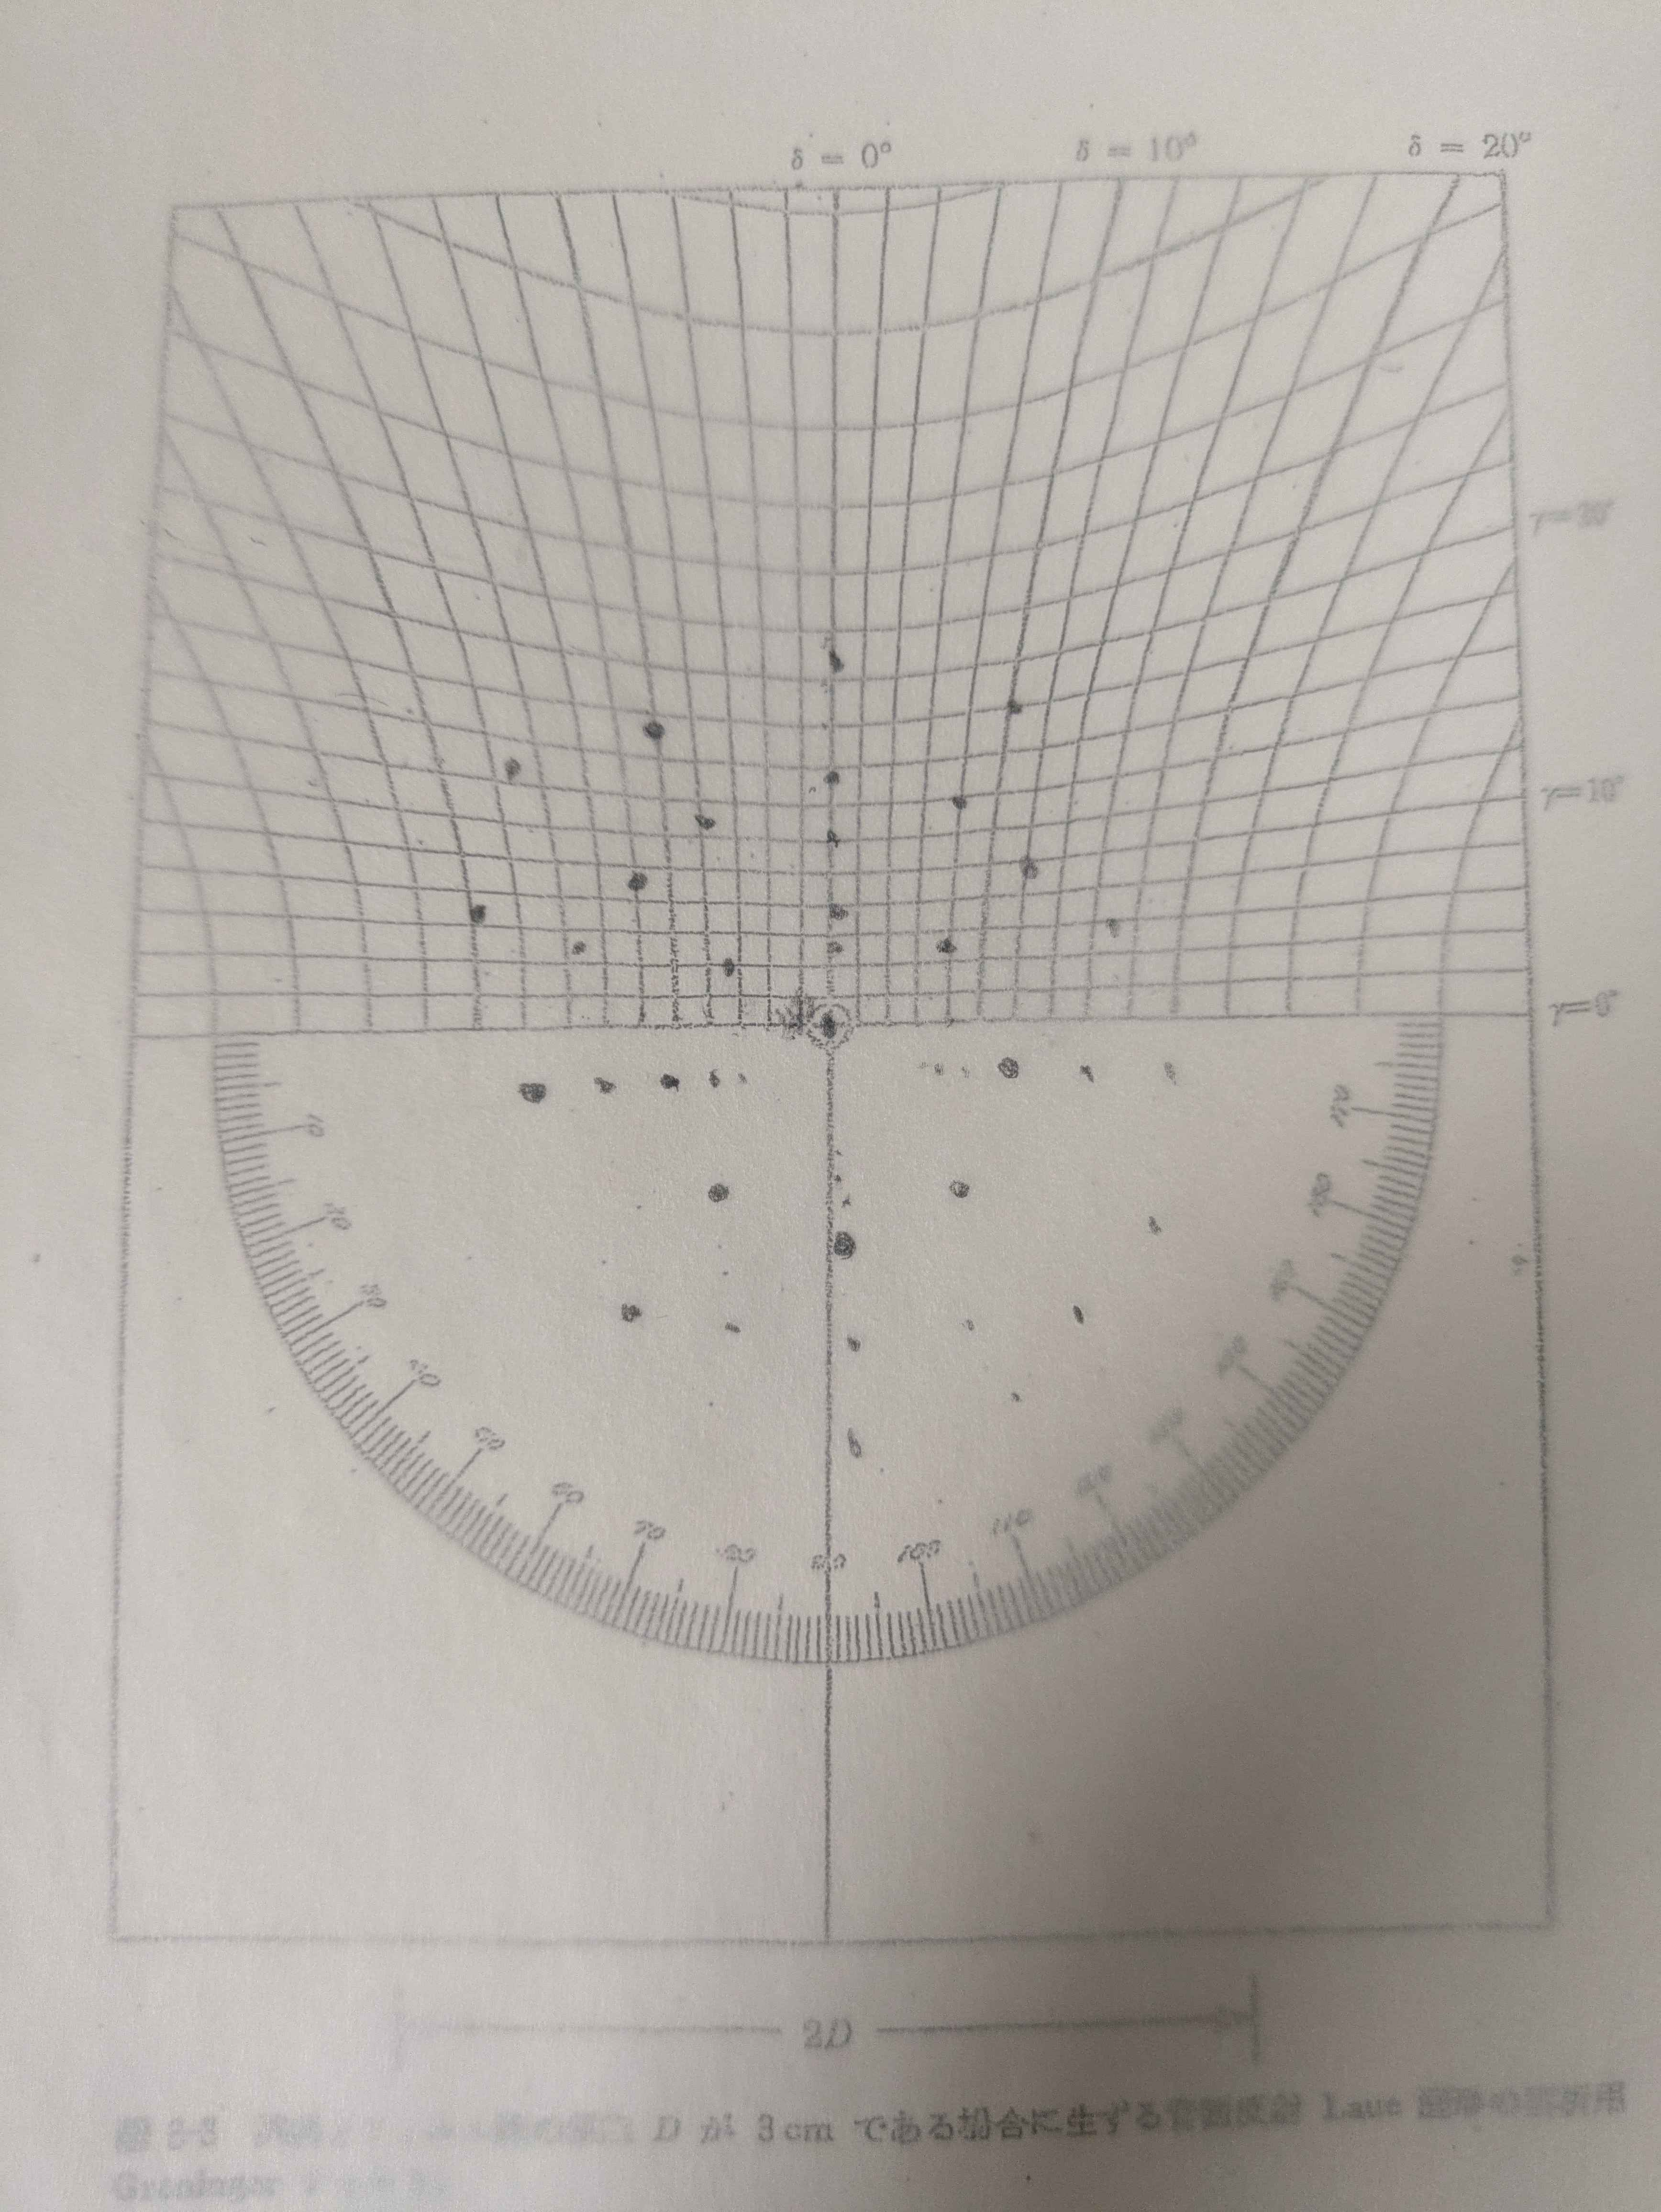
\includegraphics[width=6cm]{001_gren.jpg}
  \caption{001型結晶のグレニンガーチャート}
\end{figure}

\subsubsection{投影図}
ウルフネットを用いて出した結晶面の投影図および、各点の指数は以下のようになった。
\begin{figure}[H]
  \centering
  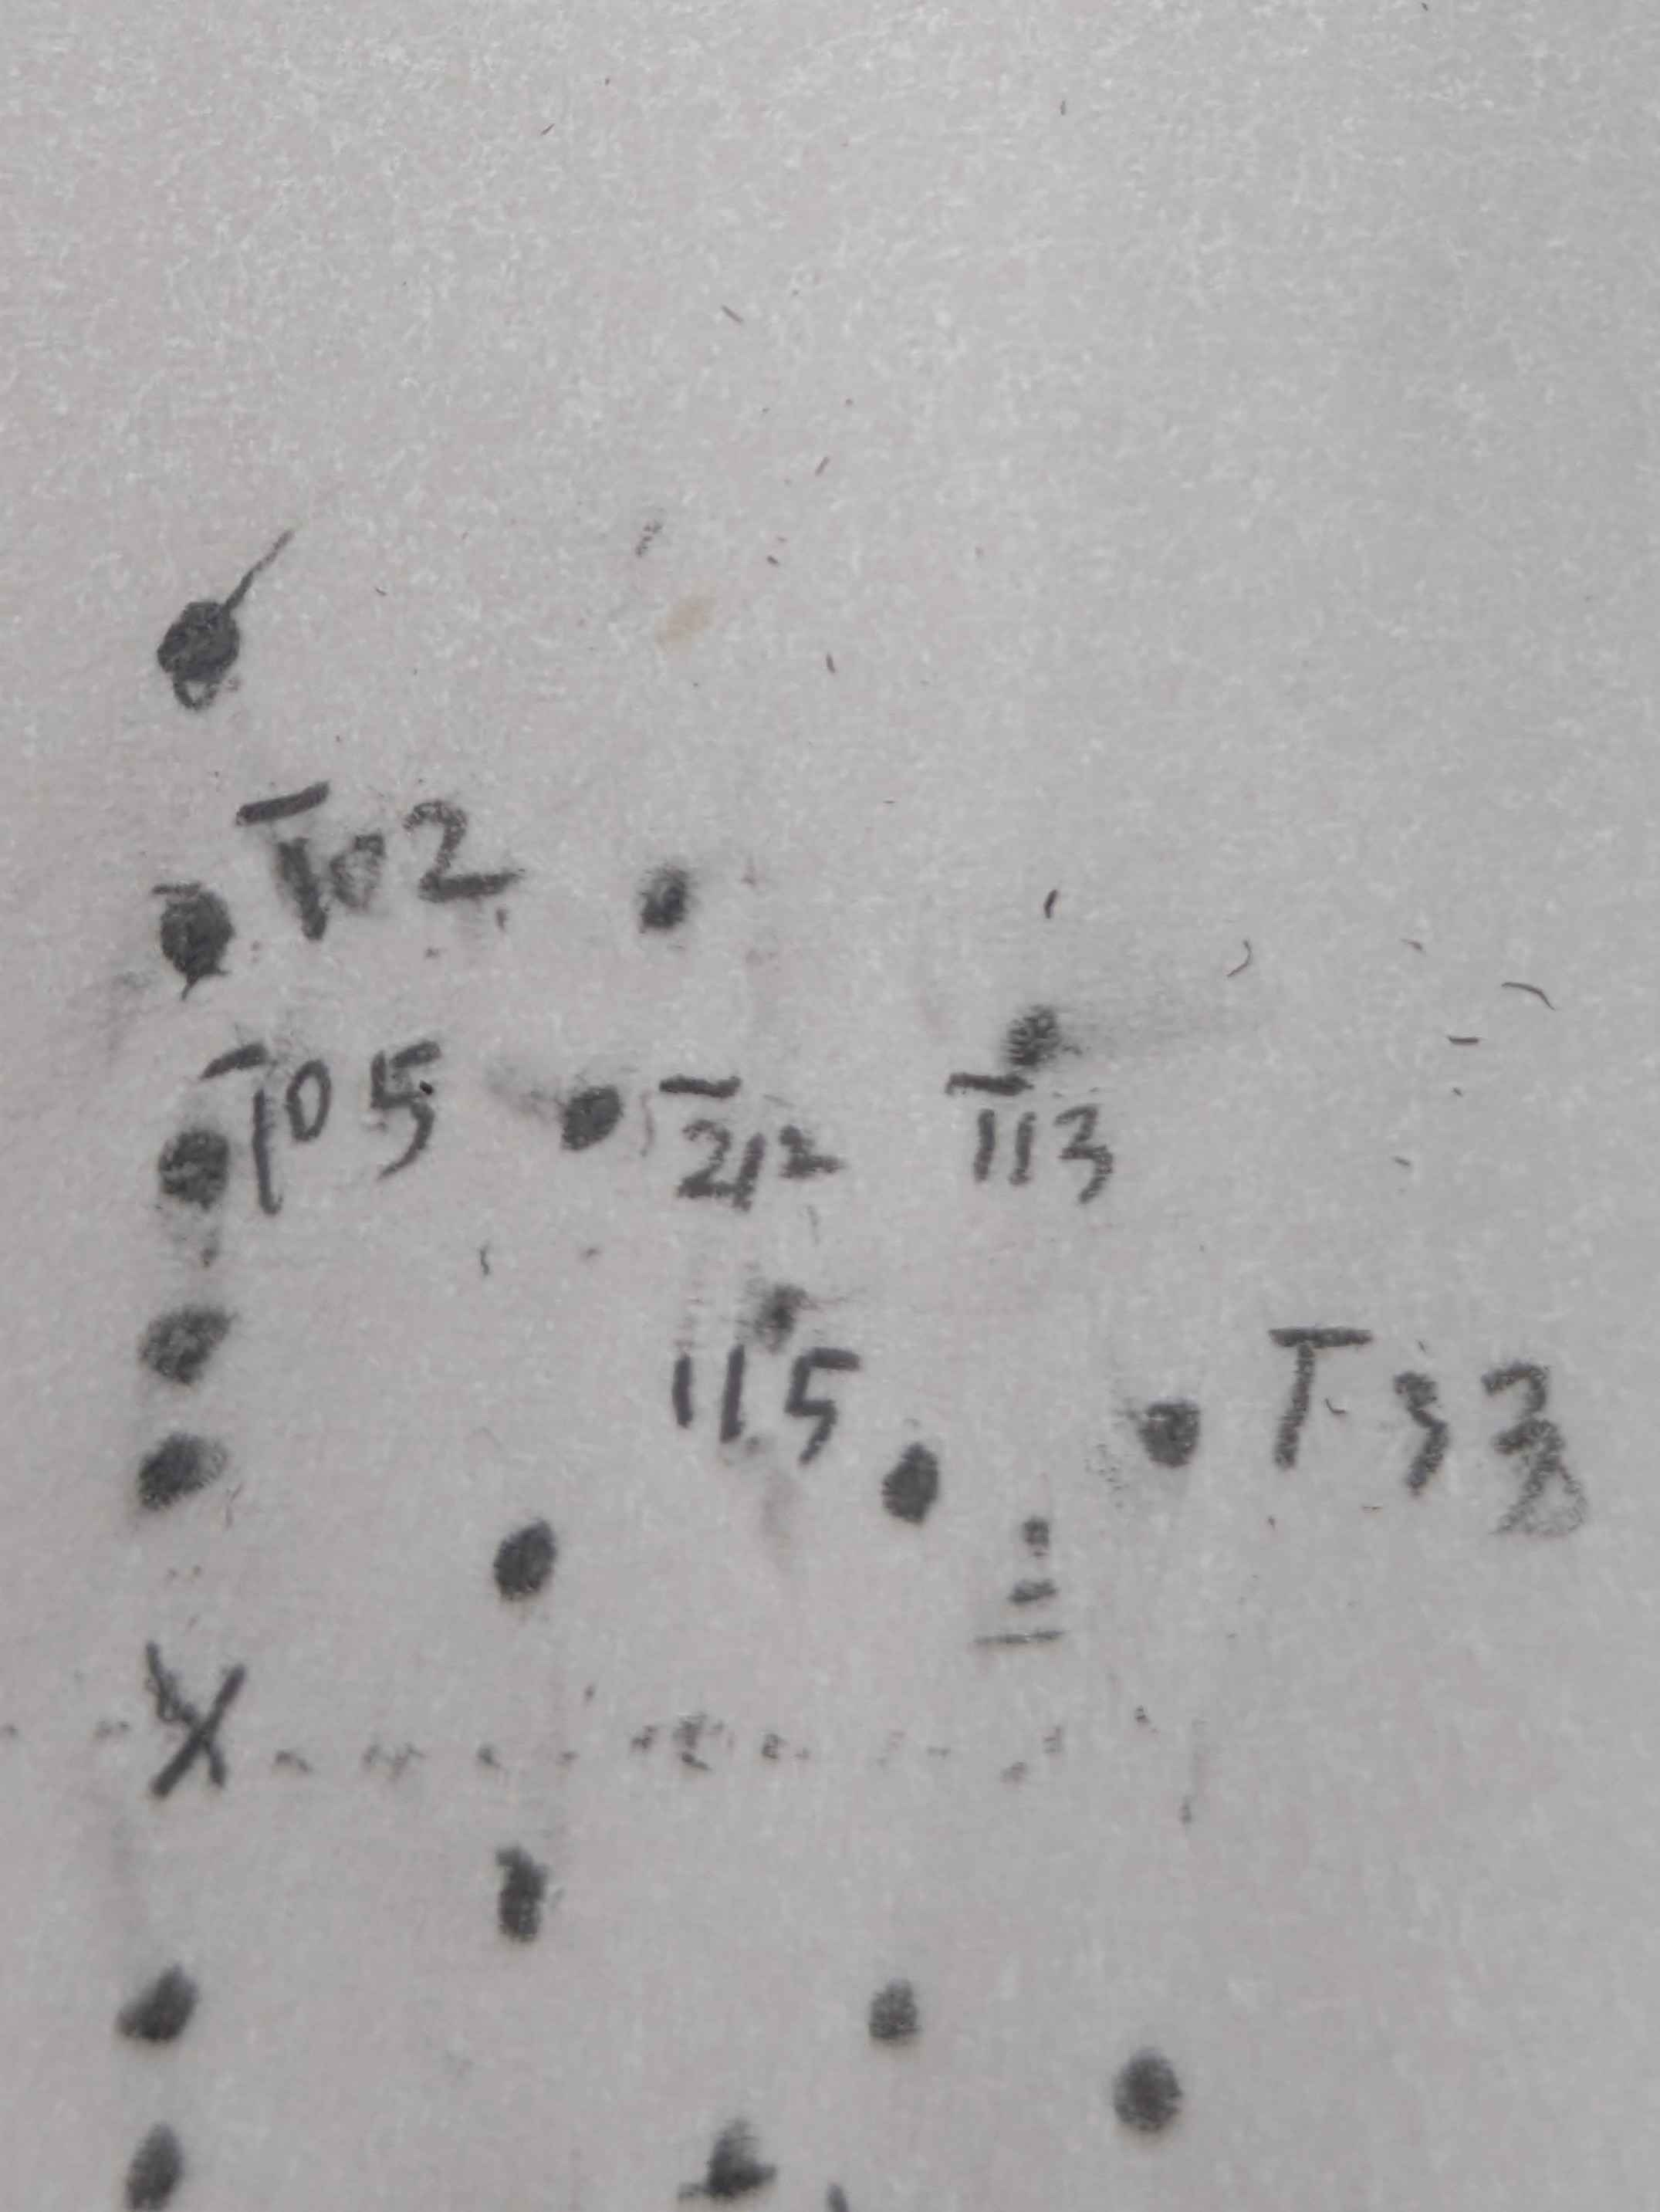
\includegraphics[width=6cm]{001_wulf.jpg}
  \caption{001型結晶の投影図}
\end{figure}
これと、標準投影図を見比べると、たしかに001型結晶であることがわかる。




\begin{thebibliography}{99}
  \bibitem{ref1} 北海道大学理学部物理学科, 『物理学実験』, 2024 ,p37-52
  \bibitem{ref2} カリティ, 『X線回折要論』, 1980, p67-69
  \bibitem{ref3} 小橋 眞,講義ノート, \url{https://www.material.nagoya-u.ac.jp/kobashi_lab/img/file47.pdf}
\end{thebibliography}

\end{document}